\documentclass[12pt,a4paper]{article}

\usepackage[a4paper,text={16.5cm,25.2cm},centering]{geometry}
\usepackage{lmodern}
\usepackage{amssymb,amsmath}
\usepackage{bm}
\usepackage{graphicx}
\usepackage{microtype}
\usepackage{hyperref}
\setlength{\parindent}{0pt}
\setlength{\parskip}{1.2ex}

\hypersetup
       {   pdfauthor = { Marco Fasondini },
           pdftitle={ foo },
           colorlinks=TRUE,
           linkcolor=black,
           citecolor=blue,
           urlcolor=blue
       }




\usepackage{upquote}
\usepackage{listings}
\usepackage{xcolor}
\lstset{
    basicstyle=\ttfamily\footnotesize,
    upquote=true,
    breaklines=true,
    breakindent=0pt,
    keepspaces=true,
    showspaces=false,
    columns=fullflexible,
    showtabs=false,
    showstringspaces=false,
    escapeinside={(*@}{@*)},
    extendedchars=true,
}
\newcommand{\HLJLt}[1]{#1}
\newcommand{\HLJLw}[1]{#1}
\newcommand{\HLJLe}[1]{#1}
\newcommand{\HLJLeB}[1]{#1}
\newcommand{\HLJLo}[1]{#1}
\newcommand{\HLJLk}[1]{\textcolor[RGB]{148,91,176}{\textbf{#1}}}
\newcommand{\HLJLkc}[1]{\textcolor[RGB]{59,151,46}{\textit{#1}}}
\newcommand{\HLJLkd}[1]{\textcolor[RGB]{214,102,97}{\textit{#1}}}
\newcommand{\HLJLkn}[1]{\textcolor[RGB]{148,91,176}{\textbf{#1}}}
\newcommand{\HLJLkp}[1]{\textcolor[RGB]{148,91,176}{\textbf{#1}}}
\newcommand{\HLJLkr}[1]{\textcolor[RGB]{148,91,176}{\textbf{#1}}}
\newcommand{\HLJLkt}[1]{\textcolor[RGB]{148,91,176}{\textbf{#1}}}
\newcommand{\HLJLn}[1]{#1}
\newcommand{\HLJLna}[1]{#1}
\newcommand{\HLJLnb}[1]{#1}
\newcommand{\HLJLnbp}[1]{#1}
\newcommand{\HLJLnc}[1]{#1}
\newcommand{\HLJLncB}[1]{#1}
\newcommand{\HLJLnd}[1]{\textcolor[RGB]{214,102,97}{#1}}
\newcommand{\HLJLne}[1]{#1}
\newcommand{\HLJLneB}[1]{#1}
\newcommand{\HLJLnf}[1]{\textcolor[RGB]{66,102,213}{#1}}
\newcommand{\HLJLnfm}[1]{\textcolor[RGB]{66,102,213}{#1}}
\newcommand{\HLJLnp}[1]{#1}
\newcommand{\HLJLnl}[1]{#1}
\newcommand{\HLJLnn}[1]{#1}
\newcommand{\HLJLno}[1]{#1}
\newcommand{\HLJLnt}[1]{#1}
\newcommand{\HLJLnv}[1]{#1}
\newcommand{\HLJLnvc}[1]{#1}
\newcommand{\HLJLnvg}[1]{#1}
\newcommand{\HLJLnvi}[1]{#1}
\newcommand{\HLJLnvm}[1]{#1}
\newcommand{\HLJLl}[1]{#1}
\newcommand{\HLJLld}[1]{\textcolor[RGB]{148,91,176}{\textit{#1}}}
\newcommand{\HLJLs}[1]{\textcolor[RGB]{201,61,57}{#1}}
\newcommand{\HLJLsa}[1]{\textcolor[RGB]{201,61,57}{#1}}
\newcommand{\HLJLsb}[1]{\textcolor[RGB]{201,61,57}{#1}}
\newcommand{\HLJLsc}[1]{\textcolor[RGB]{201,61,57}{#1}}
\newcommand{\HLJLsd}[1]{\textcolor[RGB]{201,61,57}{#1}}
\newcommand{\HLJLsdB}[1]{\textcolor[RGB]{201,61,57}{#1}}
\newcommand{\HLJLsdC}[1]{\textcolor[RGB]{201,61,57}{#1}}
\newcommand{\HLJLse}[1]{\textcolor[RGB]{59,151,46}{#1}}
\newcommand{\HLJLsh}[1]{\textcolor[RGB]{201,61,57}{#1}}
\newcommand{\HLJLsi}[1]{#1}
\newcommand{\HLJLso}[1]{\textcolor[RGB]{201,61,57}{#1}}
\newcommand{\HLJLsr}[1]{\textcolor[RGB]{201,61,57}{#1}}
\newcommand{\HLJLss}[1]{\textcolor[RGB]{201,61,57}{#1}}
\newcommand{\HLJLssB}[1]{\textcolor[RGB]{201,61,57}{#1}}
\newcommand{\HLJLnB}[1]{\textcolor[RGB]{59,151,46}{#1}}
\newcommand{\HLJLnbB}[1]{\textcolor[RGB]{59,151,46}{#1}}
\newcommand{\HLJLnfB}[1]{\textcolor[RGB]{59,151,46}{#1}}
\newcommand{\HLJLnh}[1]{\textcolor[RGB]{59,151,46}{#1}}
\newcommand{\HLJLni}[1]{\textcolor[RGB]{59,151,46}{#1}}
\newcommand{\HLJLnil}[1]{\textcolor[RGB]{59,151,46}{#1}}
\newcommand{\HLJLnoB}[1]{\textcolor[RGB]{59,151,46}{#1}}
\newcommand{\HLJLoB}[1]{\textcolor[RGB]{102,102,102}{\textbf{#1}}}
\newcommand{\HLJLow}[1]{\textcolor[RGB]{102,102,102}{\textbf{#1}}}
\newcommand{\HLJLp}[1]{#1}
\newcommand{\HLJLc}[1]{\textcolor[RGB]{153,153,119}{\textit{#1}}}
\newcommand{\HLJLch}[1]{\textcolor[RGB]{153,153,119}{\textit{#1}}}
\newcommand{\HLJLcm}[1]{\textcolor[RGB]{153,153,119}{\textit{#1}}}
\newcommand{\HLJLcp}[1]{\textcolor[RGB]{153,153,119}{\textit{#1}}}
\newcommand{\HLJLcpB}[1]{\textcolor[RGB]{153,153,119}{\textit{#1}}}
\newcommand{\HLJLcs}[1]{\textcolor[RGB]{153,153,119}{\textit{#1}}}
\newcommand{\HLJLcsB}[1]{\textcolor[RGB]{153,153,119}{\textit{#1}}}
\newcommand{\HLJLg}[1]{#1}
\newcommand{\HLJLgd}[1]{#1}
\newcommand{\HLJLge}[1]{#1}
\newcommand{\HLJLgeB}[1]{#1}
\newcommand{\HLJLgh}[1]{#1}
\newcommand{\HLJLgi}[1]{#1}
\newcommand{\HLJLgo}[1]{#1}
\newcommand{\HLJLgp}[1]{#1}
\newcommand{\HLJLgs}[1]{#1}
\newcommand{\HLJLgsB}[1]{#1}
\newcommand{\HLJLgt}[1]{#1}



\def\qqand{\qquad\hbox{and}\qquad}
\def\qqfor{\qquad\hbox{for}\qquad}
\def\qqas{\qquad\hbox{as}\qquad}
\def\half{ {1 \over 2} }
\def\D{ {\rm d} }
\def\I{ {\rm i} }
\def\E{ {\rm e} }
\def\C{ {\mathbb C} }
\def\R{ {\mathbb R} }
\def\bbR{ {\mathbb R} }
\def\H{ {\mathbb H} }
\def\Z{ {\mathbb Z} }
\def\CC{ {\cal C} }
\def\FF{ {\cal F} }
\def\HH{ {\cal H} }
\def\LL{ {\cal L} }
\def\vc#1{ {\mathbf #1} }
\def\bbC{ {\mathbb C} }



\def\fR{ f_{\rm R} }
\def\fL{ f_{\rm L} }

\def\qqqquad{\qquad\qquad}
\def\qqwhere{\qquad\hbox{where}\qquad}
\def\Res_#1{\underset{#1}{\rm Res}\,}
\def\sech{ {\rm sech}\, }
\def\acos{ {\rm acos}\, }
\def\asin{ {\rm asin}\, }
\def\atan{ {\rm atan}\, }
\def\Ei{ {\rm Ei}\, }
\def\upepsilon{\varepsilon}


\def\Xint#1{ \mathchoice
   {\XXint\displaystyle\textstyle{#1} }%
   {\XXint\textstyle\scriptstyle{#1} }%
   {\XXint\scriptstyle\scriptscriptstyle{#1} }%
   {\XXint\scriptscriptstyle\scriptscriptstyle{#1} }%
   \!\int}
\def\XXint#1#2#3{ {\setbox0=\hbox{$#1{#2#3}{\int}$}
     \vcenter{\hbox{$#2#3$}}\kern-.5\wd0} }
\def\ddashint{\Xint=}
\def\dashint{\Xint-}
% \def\dashint
\def\infdashint{\dashint_{-\infty}^\infty}




\def\addtab#1={#1\;&=}
\def\ccr{\\\addtab}
\def\ip<#1>{\left\langle{#1}\right\rangle}
\def\dx{\D x}
\def\dt{\D t}
\def\dz{\D z}
\def\ds{\D s}

\def\rR{ {\rm R} }
\def\rL{ {\rm L} }

\def\norm#1{\left\| #1 \right\|}

\def\pr(#1){\left({#1}\right)}
\def\br[#1]{\left[{#1}\right]}

\def\abs#1{\left|{#1}\right|}
\def\fpr(#1){\!\pr({#1})}

\def\sopmatrix#1{ \begin{pmatrix}#1\end{pmatrix} }

\def\endash{–}
\def\emdash{—}
\def\mdblksquare{\blacksquare}
\def\lgblksquare{\blacksquare}
\def\scre{\E}
\def\mapengine#1,#2.{\mapfunction{#1}\ifx\void#2\else\mapengine #2.\fi }

\def\map[#1]{\mapengine #1,\void.}

\def\mapenginesep_#1#2,#3.{\mapfunction{#2}\ifx\void#3\else#1\mapengine #3.\fi }

\def\mapsep_#1[#2]{\mapenginesep_{#1}#2,\void.}


\def\vcbr[#1]{\pr(#1)}


\def\bvect[#1,#2]{
{
\def\dots{\cdots}
\def\mapfunction##1{\ | \  ##1}
	\sopmatrix{
		 \,#1\map[#2]\,
	}
}
}



\def\vect[#1]{
{\def\dots{\ldots}
	\vcbr[{#1}]
} }

\def\vectt[#1]{
{\def\dots{\ldots}
	\vect[{#1}]^{\top}
} }

\def\Vectt[#1]{
{
\def\mapfunction##1{##1 \cr}
\def\dots{\vdots}
	\begin{pmatrix}
		\map[#1]
	\end{pmatrix}
} }

\def\addtab#1={#1\;&=}
\def\ccr{\\\addtab}

\def\questionequals{= \!\!\!\!\!\!{\scriptstyle ? \atop }\,\,\,}

\def\Ei{\rm Ei\,}

\begin{document}

\section{Chapter 3: Chebyshev methods for non-periodic functions}
Here we discuss:

\begin{itemize}
\item[1. ] Why high-degree polynomial interpolation in equally spaced points typically give poor approximations of functions


\item[2. ] Why high-degree polynomial interpolants in unequally spaced points are typically excellent approximants of functions


\item[3. ] Chebyshev polynomials


\item[4. ] The connection between Chebyshev and Fourier series


\item[5. ] Computing Chebyshev interpolants and their derivatives with the FFT


\item[6. ] The solution of the wave equation using the method of separation of variables


\item[7. ] The numerical solution of the wave equation using a combination of finite differences and Chebyshev interpolants


\item[8. ] The accuracy of Chebyshev interpolants and their derivatives

\end{itemize}
In the previous chapter we learned that smooth periodic functions and their derivatives can be well approximated by trigonometric interpolants:

\[
f(x) \approx p_n(x) =  \sum_{k=-(n-1)/2}^{(n-1)/2} \tilde{c}_k^n{\rm e}^{{\rm i}kx}.
\]
We also learnt that there are fast algorithms for mapping function values to coeffients and vice versa and for differentiation.  We saw how Fourier approximation methods could be used to compute an approximate solution to a PDE.

Here we'll learn that smooth \emph{non-periodic} functions and their derivatives can be accurately approximated by expansions in Chebyshev polynomials,

\[
f(x) \approx \sum_{k = 0}^{n}  \tilde{b}_k^n T_k(x).
\]
We'll see that Chebyshev expansions are Fourier expansions in disguise and therefore we can devise efficient approximation methods for PDEs with Chebyshev polynomials that use the FFT. 

\subsection{The Runge phenomenon}
Suppose we want to approximate the function $f(x) = \frac{1}{1 + 25x^2}$ (known as the Runge function) on the interval $x \in[-1, 1]$.  We know that a trigonometric interpolant will not converge very fast to $f$.  Instead, we approximate $f$ by a polynomial interpolant that interpolates $f$ at $n+1$ \emph{equally spaced} points on $[-1, 1]$.  One method to compute the interpolating polynomial is to use the formula for the Lagrange interpolating polynomial that we learned about in Chapter 1.  Instead, here we use the following "quick and dirty" method, based on inverting the Vandermonde matrix. 

Let the unique polynomial of degree $\leq n$ that interpolates $f$ at the distinct points $x_0, \ldots, x_{n}$ be denoted by $p_{n+1}(x)$, then we can express $p_{n+1}(x)$ in the monomial basis (as opposed to the Lagrange basis) as 

\[
p_{n+1}(x) = c_0 + c_1 x + \cdots + c_nx^n,
\]
and since $p_{n+1}(x_j) = f(x_j)$ for $j = 0, \ldots, n$, we have that

\[
\underbrace{\begin{bmatrix}
                    f(x_0) \\
                    \vdots \\
                    f(x_n)
                    \end{bmatrix}}_{\mathbf{f}} = 
\underbrace{ \begin{bmatrix}
                    p_{n+1}(x_0) \\
                    \vdots \\
                    p_{n+1}(x_n)
                    \end{bmatrix}}_{\mathbf{p}} = 
\begin{bmatrix} 1 & x_0 & \ensuremath{\cdots} & x_0^{n} \\
                    \ensuremath{\vdots} & \ensuremath{\vdots} & \ensuremath{\ddots} & \ensuremath{\vdots} \\
                    1 & x_n & \ensuremath{\cdots} & x_n^{n}
                    \end{bmatrix}
                    \underbrace{\begin{bmatrix}
                    c_0 \\
                    \vdots \\
                    c_n
                    \end{bmatrix}}_{\mathbf{c}}
\]
\textbf{Definition (Vandermonde)} The \emph{Vandermonde matrix} associated with $n+1$ distinct points $x_0,\ensuremath{\ldots},x_n \ensuremath{\in} \ensuremath{\bbR}$ is the matrix

\[
V := \begin{bmatrix} 1 & x_0 & \ensuremath{\cdots} & x_0^{n} \\
                    \ensuremath{\vdots} & \ensuremath{\vdots} & \ensuremath{\ddots} & \ensuremath{\vdots} \\
                    1 & x_n & \ensuremath{\cdots} & x_n^{n}
                    \end{bmatrix}.
\]
It can be shown that $V$ is non-singular, hence we can compute the coefficients $c_0, \ldots, c_n$ by solving the linear system $V\mathbf{c} = \mathbf{f}$


\begin{lstlisting}
(*@\HLJLk{using}@*) (*@\HLJLn{Plots}@*)(*@\HLJLp{,}@*) (*@\HLJLn{LinearAlgebra}@*)(*@\HLJLp{,}@*) (*@\HLJLn{ApproxFun}@*)(*@\HLJLp{,}@*) (*@\HLJLn{FFTW}@*)

(*@\HLJLn{f}@*) (*@\HLJLoB{=}@*) (*@\HLJLn{x}@*) (*@\HLJLoB{->}@*) (*@\HLJLni{1}@*)(*@\HLJLoB{/}@*)(*@\HLJLp{(}@*)(*@\HLJLni{25}@*)(*@\HLJLn{x}@*)(*@\HLJLoB{{\textasciicircum}}@*)(*@\HLJLni{2}@*) (*@\HLJLoB{+}@*) (*@\HLJLni{1}@*)(*@\HLJLp{)}@*)

(*@\HLJLcs{{\#}}@*) (*@\HLJLcs{Construct}@*) (*@\HLJLcs{an}@*) (*@\HLJLcs{interpolant}@*) (*@\HLJLcs{through}@*) (*@\HLJLcs{n}@*) (*@\HLJLcs{+}@*) (*@\HLJLcs{1}@*) (*@\HLJLcs{equally}@*) (*@\HLJLcs{spaced}@*) (*@\HLJLcs{points}@*) (*@\HLJLcs{on}@*) (*@\HLJLcs{[-1,}@*) (*@\HLJLcs{1]}@*)
(*@\HLJLn{n}@*) (*@\HLJLoB{=}@*) (*@\HLJLni{11}@*)
(*@\HLJLn{x}@*) (*@\HLJLoB{=}@*) (*@\HLJLnf{range}@*)(*@\HLJLp{(}@*)(*@\HLJLoB{-}@*)(*@\HLJLni{1}@*)(*@\HLJLp{,}@*)(*@\HLJLni{1}@*)(*@\HLJLp{;}@*)(*@\HLJLn{length}@*)(*@\HLJLoB{=}@*)(*@\HLJLn{n}@*)(*@\HLJLoB{+}@*)(*@\HLJLni{1}@*)(*@\HLJLp{)}@*)  (*@\HLJLcs{{\#}}@*) (*@\HLJLcs{n+1}@*) (*@\HLJLcs{equispaced}@*) (*@\HLJLcs{nodes}@*)  
(*@\HLJLn{xx}@*) (*@\HLJLoB{=}@*) (*@\HLJLnf{range}@*)(*@\HLJLp{(}@*)(*@\HLJLoB{-}@*)(*@\HLJLni{1}@*)(*@\HLJLp{,}@*)(*@\HLJLni{1}@*)(*@\HLJLp{;}@*)(*@\HLJLn{length}@*)(*@\HLJLoB{=}@*)(*@\HLJLni{1001}@*)(*@\HLJLp{)}@*)  (*@\HLJLcs{{\#}}@*) (*@\HLJLcs{plotting}@*) (*@\HLJLcs{grid}@*)
(*@\HLJLn{V}@*) (*@\HLJLoB{=}@*) (*@\HLJLn{x}@*) (*@\HLJLoB{.{\textasciicircum}}@*) (*@\HLJLp{(}@*)(*@\HLJLni{0}@*)(*@\HLJLoB{:}@*)(*@\HLJLn{n}@*)(*@\HLJLp{)}@*)(*@\HLJLoB{{\textquotesingle}}@*) (*@\HLJLcs{{\#}}@*) (*@\HLJLcs{Vandermonde}@*) (*@\HLJLcs{matrix}@*)
(*@\HLJLn{c}@*) (*@\HLJLoB{=}@*) (*@\HLJLn{V}@*) (*@\HLJLoB{{\textbackslash}}@*) (*@\HLJLn{f}@*)(*@\HLJLoB{.}@*)(*@\HLJLp{(}@*)(*@\HLJLn{x}@*)(*@\HLJLp{)}@*) (*@\HLJLcs{{\#}}@*) (*@\HLJLcs{coefficients}@*) (*@\HLJLcs{of}@*) (*@\HLJLcs{interpolatory}@*) (*@\HLJLcs{polynomial}@*)
(*@\HLJLn{p}@*) (*@\HLJLoB{=}@*) (*@\HLJLn{x}@*) (*@\HLJLoB{->}@*) (*@\HLJLnf{dot}@*)(*@\HLJLp{(}@*)(*@\HLJLn{c}@*)(*@\HLJLp{,}@*) (*@\HLJLn{x}@*) (*@\HLJLoB{.{\textasciicircum}}@*) (*@\HLJLp{(}@*)(*@\HLJLni{0}@*)(*@\HLJLoB{:}@*)(*@\HLJLn{n}@*)(*@\HLJLp{))}@*)  (*@\HLJLcs{{\#}}@*) (*@\HLJLcs{interpolating}@*) (*@\HLJLcs{polynomial}@*)
(*@\HLJLnf{plot}@*)(*@\HLJLp{(}@*)(*@\HLJLn{xx}@*)(*@\HLJLp{,}@*)(*@\HLJLn{f}@*)(*@\HLJLoB{.}@*)(*@\HLJLp{(}@*)(*@\HLJLn{xx}@*)(*@\HLJLp{);}@*)(*@\HLJLn{label}@*)(*@\HLJLoB{=}@*)(*@\HLJLs{"{}f(x)"{}}@*)(*@\HLJLp{)}@*)
(*@\HLJLnf{plot!}@*)(*@\HLJLp{(}@*)(*@\HLJLn{xx}@*)(*@\HLJLp{,}@*)(*@\HLJLn{p}@*)(*@\HLJLoB{.}@*)(*@\HLJLp{(}@*)(*@\HLJLn{xx}@*)(*@\HLJLp{);}@*)(*@\HLJLn{label}@*)(*@\HLJLoB{=}@*)(*@\HLJLs{"{}equispaced}@*) (*@\HLJLs{interpolant"{}}@*)(*@\HLJLp{)}@*)
(*@\HLJLnf{scatter!}@*)(*@\HLJLp{(}@*)(*@\HLJLn{x}@*)(*@\HLJLp{,}@*)(*@\HLJLn{p}@*)(*@\HLJLoB{.}@*)(*@\HLJLp{(}@*)(*@\HLJLn{x}@*)(*@\HLJLp{);}@*)(*@\HLJLn{label}@*)(*@\HLJLoB{=}@*)(*@\HLJLs{"{}samples"{}}@*)(*@\HLJLp{)}@*)
\end{lstlisting}

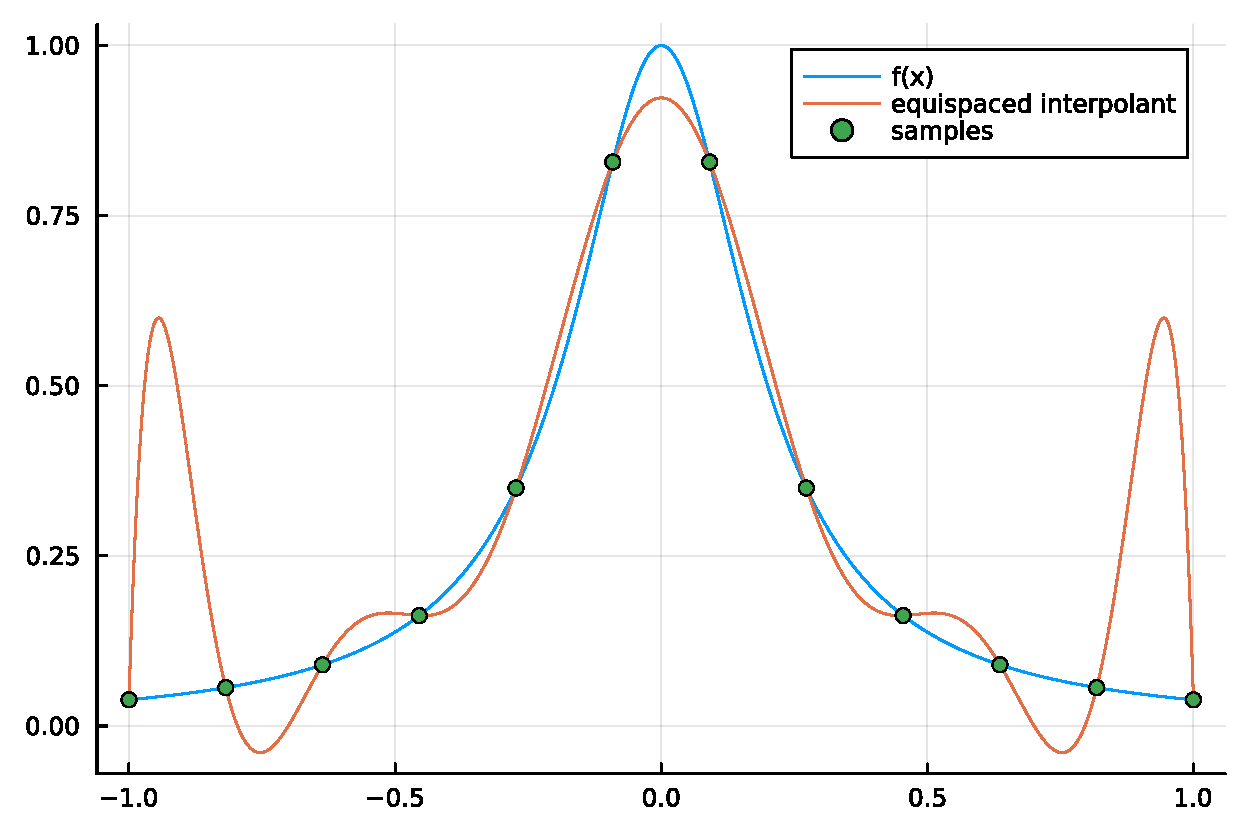
\includegraphics[width=\linewidth]{/figures/Chapter3_1_1.pdf}

The oscillations at the ends of the interval become larger as we increase $n$:


\begin{lstlisting}
(*@\HLJLn{n}@*) (*@\HLJLoB{=}@*) (*@\HLJLni{51}@*)
(*@\HLJLn{x}@*) (*@\HLJLoB{=}@*) (*@\HLJLnf{range}@*)(*@\HLJLp{(}@*)(*@\HLJLoB{-}@*)(*@\HLJLni{1}@*)(*@\HLJLp{,}@*)(*@\HLJLni{1}@*)(*@\HLJLp{;}@*)(*@\HLJLn{length}@*)(*@\HLJLoB{=}@*)(*@\HLJLn{n}@*)(*@\HLJLoB{+}@*)(*@\HLJLni{1}@*)(*@\HLJLp{)}@*)  (*@\HLJLcs{{\#}}@*) (*@\HLJLcs{n+1}@*) (*@\HLJLcs{equispaced}@*) (*@\HLJLcs{nodes}@*)  
(*@\HLJLn{V}@*) (*@\HLJLoB{=}@*) (*@\HLJLn{x}@*) (*@\HLJLoB{.{\textasciicircum}}@*) (*@\HLJLp{(}@*)(*@\HLJLni{0}@*)(*@\HLJLoB{:}@*)(*@\HLJLn{n}@*)(*@\HLJLp{)}@*)(*@\HLJLoB{{\textquotesingle}}@*) (*@\HLJLcs{{\#}}@*) (*@\HLJLcs{Vandermonde}@*) (*@\HLJLcs{matrix}@*)
(*@\HLJLn{c}@*) (*@\HLJLoB{=}@*) (*@\HLJLn{V}@*) (*@\HLJLoB{{\textbackslash}}@*) (*@\HLJLn{f}@*)(*@\HLJLoB{.}@*)(*@\HLJLp{(}@*)(*@\HLJLn{x}@*)(*@\HLJLp{)}@*) (*@\HLJLcs{{\#}}@*) (*@\HLJLcs{coefficients}@*) (*@\HLJLcs{of}@*) (*@\HLJLcs{interpolatory}@*) (*@\HLJLcs{polynomial}@*)
(*@\HLJLnf{plot}@*)(*@\HLJLp{(}@*)(*@\HLJLn{xx}@*)(*@\HLJLp{,}@*)(*@\HLJLn{f}@*)(*@\HLJLoB{.}@*)(*@\HLJLp{(}@*)(*@\HLJLn{xx}@*)(*@\HLJLp{);}@*)(*@\HLJLn{label}@*)(*@\HLJLoB{=}@*)(*@\HLJLs{"{}f(x)"{}}@*)(*@\HLJLp{,}@*)(*@\HLJLn{ylims}@*)(*@\HLJLoB{=}@*)(*@\HLJLp{(}@*)(*@\HLJLoB{-}@*)(*@\HLJLni{3}@*)(*@\HLJLp{,}@*)(*@\HLJLni{3}@*)(*@\HLJLp{))}@*)
(*@\HLJLnf{plot!}@*)(*@\HLJLp{(}@*)(*@\HLJLn{xx}@*)(*@\HLJLp{,}@*)(*@\HLJLn{p}@*)(*@\HLJLoB{.}@*)(*@\HLJLp{(}@*)(*@\HLJLn{xx}@*)(*@\HLJLp{);}@*)(*@\HLJLn{label}@*)(*@\HLJLoB{=}@*)(*@\HLJLs{"{}equispaced}@*) (*@\HLJLs{interpolant"{}}@*)(*@\HLJLp{)}@*)
(*@\HLJLnf{scatter!}@*)(*@\HLJLp{(}@*)(*@\HLJLn{x}@*)(*@\HLJLp{,}@*)(*@\HLJLn{p}@*)(*@\HLJLoB{.}@*)(*@\HLJLp{(}@*)(*@\HLJLn{x}@*)(*@\HLJLp{);}@*)(*@\HLJLn{label}@*)(*@\HLJLoB{=}@*)(*@\HLJLs{"{}samples"{}}@*)(*@\HLJLp{)}@*)
\end{lstlisting}

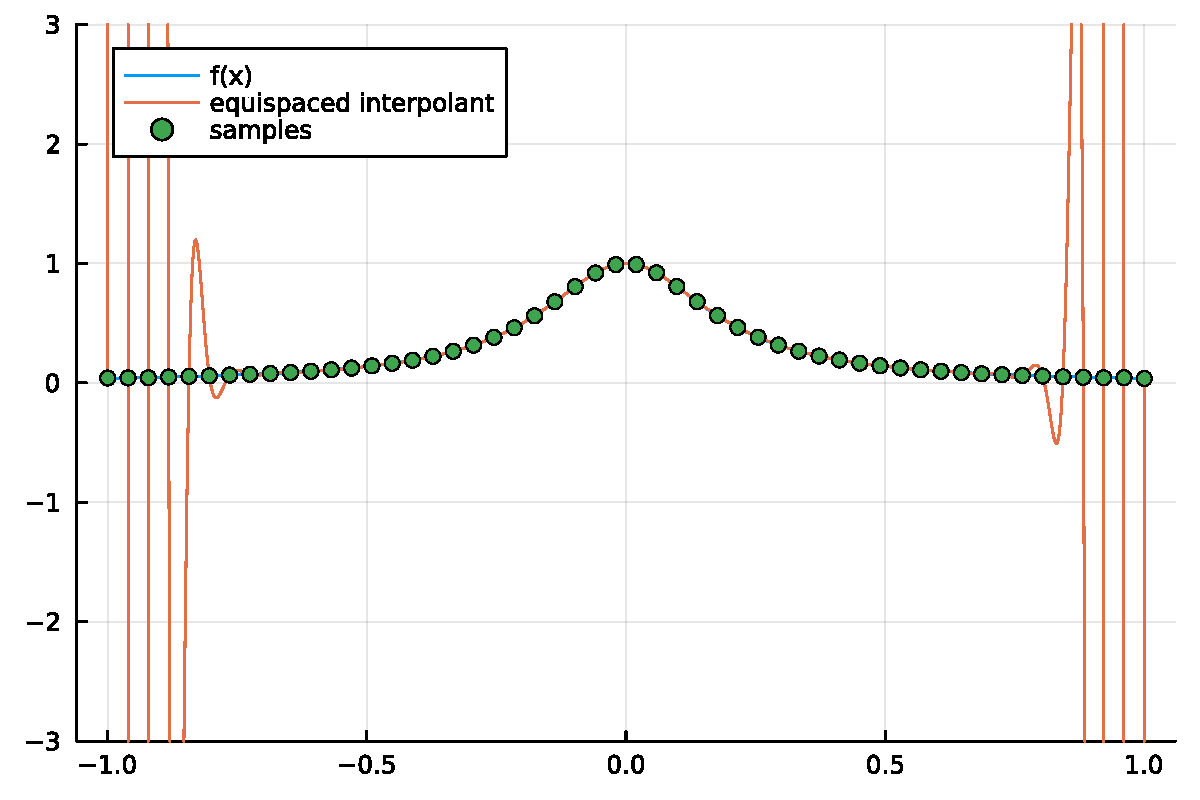
\includegraphics[width=\linewidth]{/figures/Chapter3_2_1.pdf}

These oscillations of the interpolant through equally spaced nodes is known as the \emph{Runge phenomenon} (not to be confused with the Gibbs phenomenon in Chapter 2). Equally spaced interpolation nodes is clearly not a good choice for high-degree polynomial interpolation.  Maybe the oscillations at the endpoints can be suppressed if we choose nodes that are clustered at the ends of the interval?


\begin{lstlisting}
(*@\HLJLcs{{\#}}@*) (*@\HLJLcs{Construct}@*) (*@\HLJLcs{an}@*) (*@\HLJLcs{interpolant}@*) (*@\HLJLcs{using}@*) (*@\HLJLcs{ApproxFun}@*)
(*@\HLJLn{n}@*) (*@\HLJLoB{=}@*) (*@\HLJLni{11}@*)
(*@\HLJLn{S}@*) (*@\HLJLoB{=}@*) (*@\HLJLnf{Chebyshev}@*)(*@\HLJLp{()}@*)
(*@\HLJLn{p}@*) (*@\HLJLoB{=}@*) (*@\HLJLnf{Fun}@*)(*@\HLJLp{(}@*)(*@\HLJLn{f}@*)(*@\HLJLp{,}@*)(*@\HLJLn{S}@*)(*@\HLJLp{,}@*)(*@\HLJLn{n}@*)(*@\HLJLoB{+}@*)(*@\HLJLni{1}@*)(*@\HLJLp{)}@*) (*@\HLJLcs{{\#}}@*) (*@\HLJLcs{an}@*) (*@\HLJLcs{interpolant}@*) (*@\HLJLcs{through}@*) (*@\HLJLcs{clustered}@*) (*@\HLJLcs{nodes}@*)
(*@\HLJLn{x}@*) (*@\HLJLoB{=}@*) (*@\HLJLnf{points}@*)(*@\HLJLp{(}@*)(*@\HLJLn{S}@*)(*@\HLJLp{,}@*)(*@\HLJLn{n}@*)(*@\HLJLoB{+}@*)(*@\HLJLni{1}@*)(*@\HLJLp{)}@*)  (*@\HLJLcs{{\#}}@*) (*@\HLJLcs{n+1}@*) (*@\HLJLcs{unevenly}@*) (*@\HLJLcs{spaced}@*) (*@\HLJLcs{points}@*) 
(*@\HLJLnf{plot}@*)(*@\HLJLp{(}@*)(*@\HLJLn{xx}@*)(*@\HLJLp{,}@*)(*@\HLJLn{f}@*)(*@\HLJLoB{.}@*)(*@\HLJLp{(}@*)(*@\HLJLn{xx}@*)(*@\HLJLp{);}@*)(*@\HLJLn{label}@*)(*@\HLJLoB{=}@*)(*@\HLJLs{"{}f(x)"{}}@*)(*@\HLJLp{)}@*)
(*@\HLJLnf{plot!}@*)(*@\HLJLp{(}@*)(*@\HLJLn{p}@*)(*@\HLJLp{;}@*)(*@\HLJLn{label}@*)(*@\HLJLoB{=}@*)(*@\HLJLs{"{}interpolant"{}}@*)(*@\HLJLp{)}@*)
(*@\HLJLnf{scatter!}@*)(*@\HLJLp{(}@*)(*@\HLJLn{x}@*)(*@\HLJLp{,}@*)(*@\HLJLn{p}@*)(*@\HLJLoB{.}@*)(*@\HLJLp{(}@*)(*@\HLJLn{x}@*)(*@\HLJLp{);}@*)(*@\HLJLn{label}@*)(*@\HLJLoB{=}@*)(*@\HLJLs{"{}samples"{}}@*)(*@\HLJLp{)}@*)
\end{lstlisting}

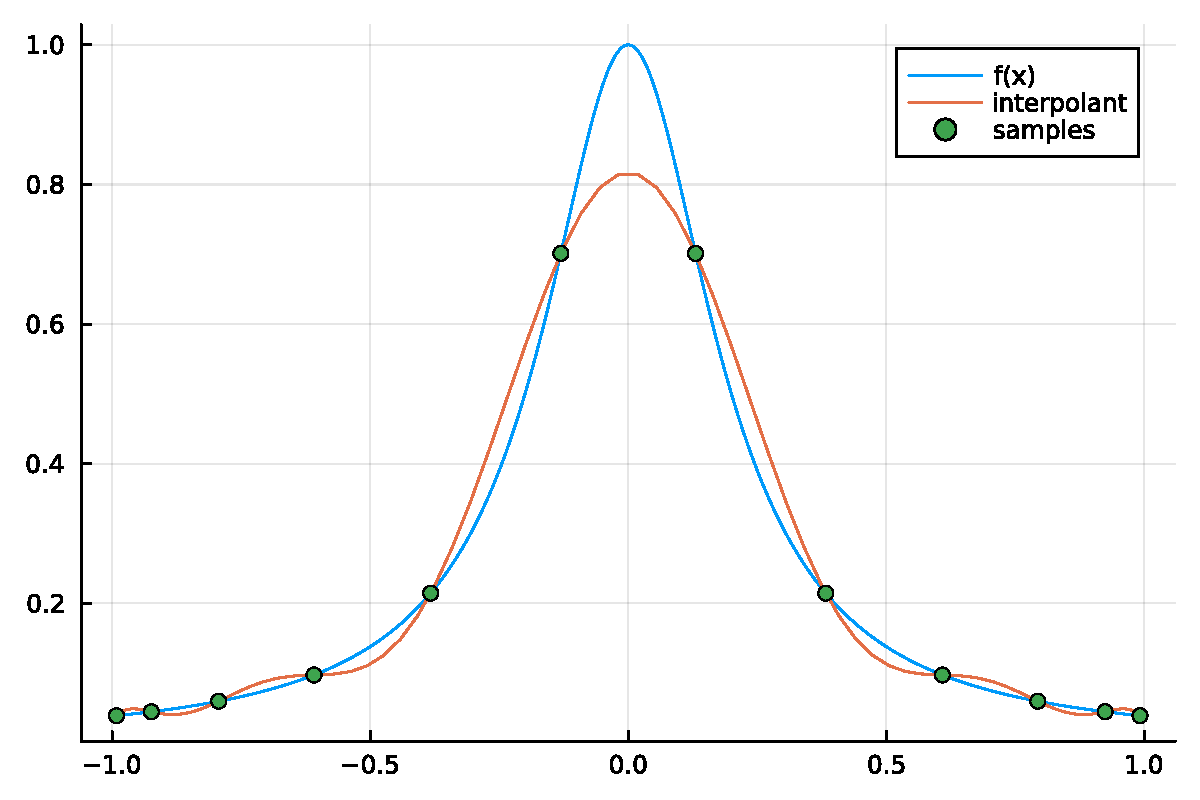
\includegraphics[width=\linewidth]{/figures/Chapter3_3_1.pdf}

In the above figure, we interpolated $f(x)$ at the roots (zeros) of a Chebyshev polynomial, which we'll learn about later.  The interpolants at the roots of the Chebyshev polynomials converge exponentially fast to $f$ on $[-1, 1]$ as $n$ (the number of interpolation nodes) increases.


\begin{lstlisting}
(*@\HLJLn{n}@*) (*@\HLJLoB{=}@*) (*@\HLJLni{31}@*)
(*@\HLJLn{S}@*) (*@\HLJLoB{=}@*) (*@\HLJLnf{Chebyshev}@*)(*@\HLJLp{()}@*)
(*@\HLJLn{p}@*) (*@\HLJLoB{=}@*) (*@\HLJLnf{Fun}@*)(*@\HLJLp{(}@*)(*@\HLJLn{f}@*)(*@\HLJLp{,}@*)(*@\HLJLn{S}@*)(*@\HLJLp{,}@*)(*@\HLJLn{n}@*)(*@\HLJLoB{+}@*)(*@\HLJLni{1}@*)(*@\HLJLp{)}@*) 
(*@\HLJLn{x}@*) (*@\HLJLoB{=}@*) (*@\HLJLnf{points}@*)(*@\HLJLp{(}@*)(*@\HLJLn{S}@*)(*@\HLJLp{,}@*)(*@\HLJLn{n}@*)(*@\HLJLoB{+}@*)(*@\HLJLni{1}@*)(*@\HLJLp{)}@*) 
(*@\HLJLnf{plot}@*)(*@\HLJLp{(}@*)(*@\HLJLn{xx}@*)(*@\HLJLp{,}@*)(*@\HLJLn{f}@*)(*@\HLJLoB{.}@*)(*@\HLJLp{(}@*)(*@\HLJLn{xx}@*)(*@\HLJLp{);}@*)(*@\HLJLn{label}@*)(*@\HLJLoB{=}@*)(*@\HLJLs{"{}f"{}}@*)(*@\HLJLp{)}@*)
(*@\HLJLnf{plot!}@*)(*@\HLJLp{(}@*)(*@\HLJLn{p}@*)(*@\HLJLp{;}@*)(*@\HLJLn{label}@*)(*@\HLJLoB{=}@*)(*@\HLJLs{"{}interpolant"{}}@*)(*@\HLJLp{)}@*)
(*@\HLJLnf{scatter!}@*)(*@\HLJLp{(}@*)(*@\HLJLn{x}@*)(*@\HLJLp{,}@*)(*@\HLJLn{p}@*)(*@\HLJLoB{.}@*)(*@\HLJLp{(}@*)(*@\HLJLn{x}@*)(*@\HLJLp{);}@*)(*@\HLJLn{label}@*)(*@\HLJLoB{=}@*)(*@\HLJLs{"{}samples"{}}@*)(*@\HLJLp{)}@*)
\end{lstlisting}

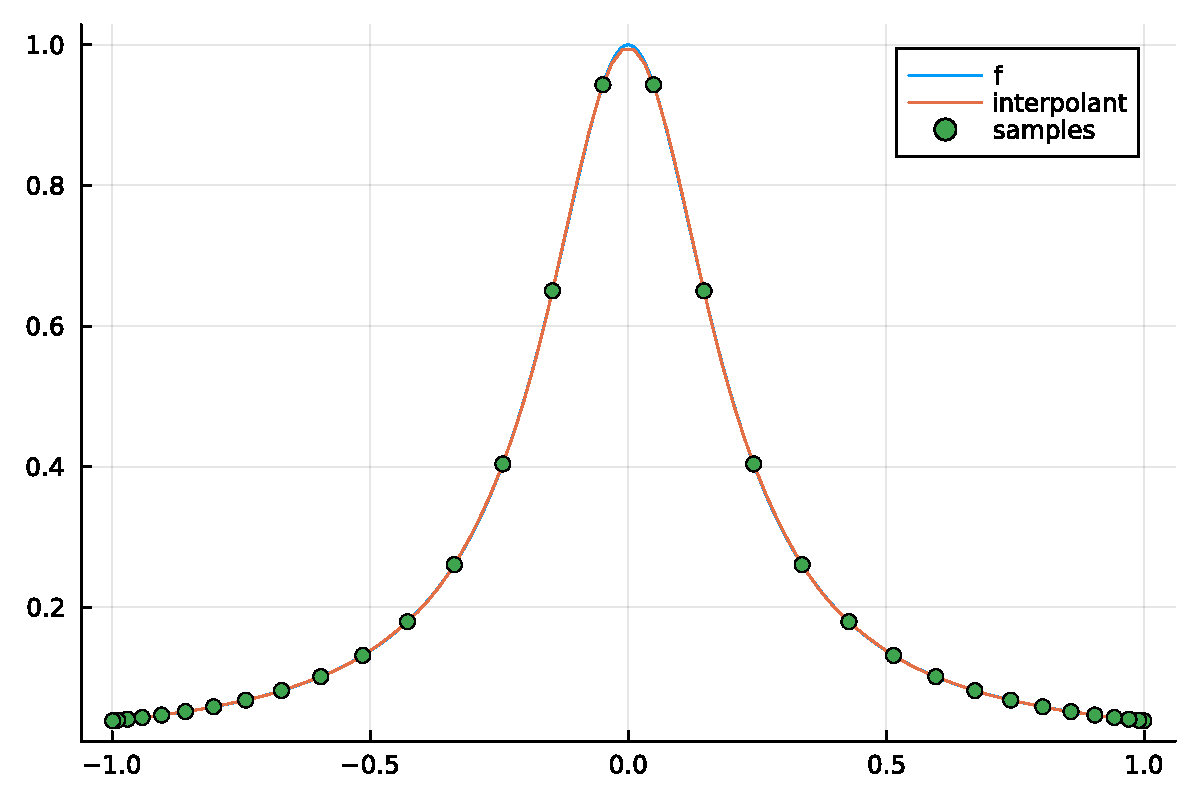
\includegraphics[width=\linewidth]{/figures/Chapter3_4_1.pdf}

Later we'll learn that interpolants at the roots of Chebyshev polynomials can be computed using the FFT ($\mathcal{O}(n\log n)$ complexity), which is much more efficient than inverting a Vandermonde matrix ($\mathcal{O}(n^3)$ complexity). 

\textbf{Remark}  An understanding of the reasons why equispaced interpolation failed for the above function and why interpolants through clustered points converged fast require tools from complex analysis and potential theory (See \emph{Approximation Theory and Approximation Practice} by L.N. Trefethen).

\subsection{An introduction to Chebyshev polynomials}
\textbf{Definition (Chebyshev polynomials of the first kind)}

\[
T_n(x) = \cos n\, {\rm acos} x, \qquad x \in [-1, 1],
\]
or in other words,

\[
T_n(\cos \theta) = \cos n \theta, \qquad \theta \in [0, \pi].
\]
\textbf{Proposition (Chebyshev three-term recurrence)}  The Chebyshev polynomials satisfy the following three-term recurrence:


\begin{align*}
xT_{n} = \frac{T_{n-1}(x) + T_{n+1}(x)}{2}, \qquad n \geq 1.
\end{align*}
\textbf{Proof}

It follows immediately from the definition that $T_0(x) = 1$, $T_{1}(x) = x$ and for $n \geq 1$

\[
x T_n(x) = \cos \ensuremath{\theta} \cos n \ensuremath{\theta} = {\cos(n-1)\ensuremath{\theta} + \cos(n+1)\ensuremath{\theta} \over 2} = {T_{n-1}(x) + T_{n+1}(x) \over 2}
\]
In other words $T_{n+1}(x) = 2x T_n(x) - T_{n-1}(x)$ for $n \geq 1$.

\[
\blacksquare
\]
\textbf{Corollary} $T_n(x)$ is a polynomial of degree precisely $n$.

Here are a few Chebyshev polynomials


\begin{lstlisting}
(*@\HLJLn{xx}@*) (*@\HLJLoB{=}@*) (*@\HLJLoB{-}@*)(*@\HLJLni{1}@*)(*@\HLJLoB{:}@*)(*@\HLJLnfB{0.01}@*)(*@\HLJLoB{:}@*)(*@\HLJLni{1}@*)
(*@\HLJLn{p}@*) (*@\HLJLoB{=}@*) (*@\HLJLnf{plot}@*)(*@\HLJLp{()}@*)
(*@\HLJLk{for}@*) (*@\HLJLn{k}@*) (*@\HLJLoB{=}@*) (*@\HLJLni{1}@*)(*@\HLJLoB{:}@*)(*@\HLJLni{4}@*)
    (*@\HLJLnf{plot!}@*)(*@\HLJLp{(}@*)(*@\HLJLn{xx}@*)(*@\HLJLp{,}@*)(*@\HLJLnf{Fun}@*)(*@\HLJLp{(}@*)(*@\HLJLnf{Chebyshev}@*)(*@\HLJLp{(),[}@*)(*@\HLJLnf{fill}@*)(*@\HLJLp{(}@*)(*@\HLJLni{0}@*)(*@\HLJLp{,}@*)(*@\HLJLn{k}@*)(*@\HLJLp{);}@*)(*@\HLJLni{1}@*)(*@\HLJLp{])}@*)(*@\HLJLoB{.}@*)(*@\HLJLp{(}@*)(*@\HLJLn{xx}@*)(*@\HLJLp{);}@*)(*@\HLJLn{label}@*)(*@\HLJLoB{=}@*)(*@\HLJLs{"{}T{\_}}@*)(*@\HLJLsi{{\$}k}@*)(*@\HLJLs{"{}}@*)(*@\HLJLp{)}@*)
(*@\HLJLk{end}@*)
(*@\HLJLn{p}@*)
\end{lstlisting}

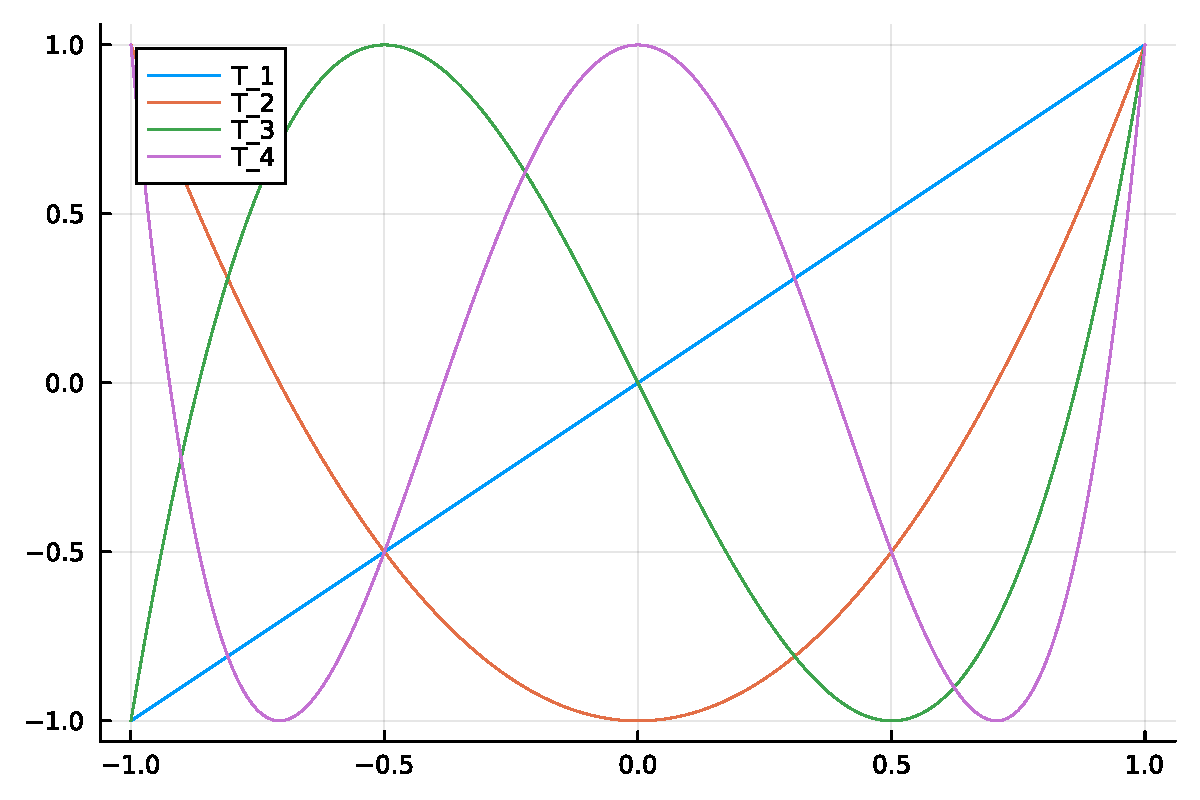
\includegraphics[width=\linewidth]{/figures/Chapter3_5_1.pdf}

In the example above, we resolved the Runge phenomenon by interpolating the function at the roots of $T_n(x)$, which are at

\[
    x_j = \cos\left(\frac{(2j+1)\pi}{2n}\right), \qquad j = 0, \ldots, n-1, 
\]
since $T_n(x_j) = \cos n\,\mathrm{acos} x_j = \cos\left(\frac{(2j+1)\pi}{2}\right) = 0$.  Later on, we shall be interested in the points

\[
x_j = \cos\left(\frac{j\pi}{n}\right), \qquad j = 0, \ldots, n, 
\]
which are the extrema (maxima and minima) of $T_{n+2}(x)$.  Notice that the roots of $T_n$ are in $(-1, 1)$, whereas the extrema of $T_{n+2}$ are in $[-1, 1]$.

\subsection{The relation between Chebyshev and Fourier series}
Suppose a function $f(x)$ has a convergent Chebyshev series for $x \in [-1, 1]$, i.e.,

\[
f(x) = \sum_{k=0}^{\infty} b_k T_k(x).
\]
Let's call the function that results from the change of variable $x = \cos \theta$, $g(\theta)$, i.e.,

\[
g(\theta) = f(\cos \theta).
\]
Notice that $g$ is an even, $2\pi$-periodic function of $\theta$.  We have that


\begin{eqnarray*}
f(x) &=& \sum_{k=0}^{\infty} b_k T_k(x) \\
  &=& \sum_{k=0}^{\infty} b_k\cos k\theta   \qquad (x = \cos \theta)  \\
  & = & g(\theta) \\
  &=& \sum_{k=0}^{\infty} b_k\left(\frac{{\rm e}^{{\rm i}k\theta} + {\rm e}^{-{\rm i}k\theta}}{2}   \right) \\
  &=& \sum_{k=-\infty}^{\infty} c_k {\rm e}^{{\rm i}k\theta}  \qquad (c_0 = b_0, c_{k} = c_{-k} = b_k/2, k\geq 1).
\end{eqnarray*}
That is, a Chebyshev series is a Fourier series in disguise! We have just proved the following result.

\textbf{Proposition (Chebyshev coefficients defined as Fourier coefficients)} If $g(\theta) = f(\cos \theta)$ can be expressed as a Fourier series, then $f(x)$ has a Chebyshev series and the Chebyshev coefficients $b_k$, $k \geq 0$ of $f(x)$ are related to the Fourier coefficients $c_k$, $k \in \mathbb{Z}$  of $g(\theta)$ as follows,

\[
b_0 = c_0, \qquad b_k = 2c_k = 2c_{-k}.
\]
where

\[
c_k = \frac{1}{2\pi}\int_{0}^{2\pi}g(\theta){\rm e}^{-{\rm i}k\theta}\,{\rm d}\theta.
\]
\textbf{Remark} We can prove that $c_{-k} = c_{k}$ for $g(\theta)$ by observing that 


\begin{eqnarray*}
c_k &=& \frac{1}{2\pi} \int_{0}^{2\pi} g(\theta){\rm e}^{-{\rm i}k\theta}\,{\rm d}\theta \\
    &=& \frac{(-1)^{k}}{2\pi} \int_{-\pi}^{\pi} g(\theta +\pi){\rm e}^{-{\rm i}k\theta}\,{\rm d}\theta \\
    &=& \frac{(-1)^{k}}{2\pi} \int_{-\pi}^{\pi} g(\theta +\pi)\left(\cos k\theta - {\rm i} \sin k\theta   \right)\,{\rm d}\theta \\
    &=& \frac{(-1)^{k}}{2\pi} \int_{-\pi}^{\pi} g(\theta +\pi) \cos k\theta \,{\rm d}\theta
\end{eqnarray*}
where we used the fact that $\sin k \theta$ is an odd function, $\cos k \theta$ is an even function and $h(\theta) := g(\theta + \pi) $ is an even function of $\theta$ because

\[
h(\theta) = g(\theta + \pi) = f(\cos(\theta+\pi)) = f(\cos(-\theta+\pi)) = g(-\theta +\pi) = h(-\theta). 
\]
Therefore if we replace $k$ with $-k$, we get the same integral and hence $c_{k} = c_{-k}$.

\subsection{The relation between Chebyshev and trigonometric interpolants}
From Chapter 2, we know that the truncated Fourier series

\[
q_{2n+1}(\theta) = \sum_{k=-n}^{n} \tilde{c}_k^{2n+1} {\rm e}^{{\rm i}k\theta},
\]
where

\[
\tilde{c}_k^{2n+1} = \frac{1}{2n+1}\sum_{j = 0}^{2n} g(\theta_j) {\rm e}^{-{\rm i}k\theta_j}, \qquad k = -n, \ldots, n, \qquad \theta_{j} = \frac{2\pi j}{2n+1},\qquad j = 0, \ldots, 2n,
\]
interpolates $g(\theta)$ at $\theta = \theta_j$, $j = 0, \ldots, 2n$.  Using parity arguments (as we did when we proved that $c_{k} = c_{-k}$ for $g(\theta)$), we can show that $\tilde{c}_k^{2n+1} = \tilde{c}_{-k}^{2n+1}$. Therefore,


\begin{eqnarray*}
q_{2n+1}(\theta) &=& \tilde{c}_0^{2n+1}+ \sum_{k=1}^{n} \tilde{c}_k^{2n+1}\left( {\rm e}^{{\rm i}k\theta} + {\rm e}^{-{\rm i}k\theta} \right) \\
&=&  \tilde{c}_0^{2n+1} + 2\sum_{k=1}^{n} \tilde{c}_k^{2n+1}\cos k\theta \\
&=&  \tilde{c}_0^{2n+1} + 2\sum_{k=1}^{n} \tilde{c}_k^{2n+1} T_k(x) \qquad (x = \cos\theta) \\
&:=& p_{n+1}(x)
\end{eqnarray*}
from which we get the following result.

\textbf{Proposition (Chebyshev polynomial interpolant constructed from a trigonometric interpolant)} The polynomial of degree $\leq n$ defined by 

\[
p_{n+1}(x) = \sum_{k=0}^{n} \tilde{b}_k^nT_k(x) 
\]
where

\[
\tilde{b}_0^n = \tilde{c}_0^{2n+1}, \qquad \tilde{b}_k^n = 2\tilde{c}_k^{2n+1}  = 2\tilde{c}_{-k}^{2n+1}
\]
interpolates $f(x)$  at $x_{j}$, where

\[
x_j = \cos\left( \frac{2\pi j}{2n + 1}  \right), \qquad j = 0, \ldots, n
\]
\textbf{Proof} Since 

\[
q_{2n+1}(\theta_j) = g(\theta_j), \qquad \theta_j = \frac{2\pi j}{2n+ 1}, \qquad j = 0, \ldots, 2n
\]
and $q_{2n}(\theta) = p_{2n+1}(\cos \theta) = p_{2n+1}(x)$ where $x = \cos\theta$, it follows that

\[
p_{2n+1}(x_j) =p_{2n+1}(\cos \theta_j) = q_{2n+1}(\theta_j) = g(\theta_j) = f(\cos\theta_j) = f(x_j), \qquad j = 0, \ldots, 2n.
\]
The result follows by noting that only $n+1$ of the $2n+1$ points $x_j$, $j = 0, \ldots, 2n$ are distinct because

\[
x_{n} = \cos\left( \frac{2\pi n}{2n + 1}  \right)= \cos\left( \pi - \frac{\pi}{2n + 1}  \right) =  \cos\left( \pi + \frac{\pi}{2n + 1}  \right) = x_{n+1}
\]
and similarly $x_{n-1} = x_{n+2}$, $\ldots$, $x_1 = x_{2n}$.  $\blacksquare$

We refer to $p_{n+1}(x) = \sum_{k=0}^{n} \tilde{b}_k^nT_k(x)$ as a Chebyshev interpolant of $f(x)$ and the $\tilde{b}_k^n$ are the approximate Chebyshev coefficients of the the function $f$ we are approximating.

Recall that the approximate Fourier coefficients $\tilde{c}^{2n+1}_k$ can be computed with the FFT, hence we can compute the coefficients $\tilde{b}^n_k$ of a Chebyshev interpolant with the FFT.  We can use the (inverse) FFT to map the coefficients $\tilde{b}^n_k$ to the function values $f(x_j)$. Here's an example:


\begin{lstlisting}
(*@\HLJLcs{{\#}}@*) (*@\HLJLcs{Use}@*) (*@\HLJLcs{the}@*) (*@\HLJLcs{FFT}@*) (*@\HLJLcs{to}@*) (*@\HLJLcs{compute}@*) (*@\HLJLcs{the}@*) (*@\HLJLcs{approximate}@*) (*@\HLJLcs{Chebyshev}@*) (*@\HLJLcs{coefficients}@*) (*@\HLJLcs{of}@*) (*@\HLJLcs{the}@*) (*@\HLJLcs{Runge}@*) (*@\HLJLcs{function}@*)
(*@\HLJLn{g}@*) (*@\HLJLoB{=}@*) (*@\HLJLn{\ensuremath{\theta}}@*) (*@\HLJLoB{->}@*) (*@\HLJLnf{f}@*)(*@\HLJLp{(}@*)(*@\HLJLnf{cos}@*)(*@\HLJLp{(}@*)(*@\HLJLn{\ensuremath{\theta}}@*)(*@\HLJLp{))}@*)
(*@\HLJLn{n}@*) (*@\HLJLoB{=}@*) (*@\HLJLni{200}@*)
(*@\HLJLn{\ensuremath{\theta}}@*) (*@\HLJLoB{=}@*) (*@\HLJLnf{range}@*)(*@\HLJLp{(}@*)(*@\HLJLni{0}@*)(*@\HLJLp{,}@*)(*@\HLJLni{2}@*)(*@\HLJLn{\ensuremath{\pi}}@*)(*@\HLJLp{;}@*)(*@\HLJLn{length}@*)(*@\HLJLoB{=}@*) (*@\HLJLni{2}@*)(*@\HLJLn{n}@*)(*@\HLJLoB{+}@*)(*@\HLJLni{2}@*)(*@\HLJLp{)[}@*)(*@\HLJLni{1}@*)(*@\HLJLoB{:}@*)(*@\HLJLk{end}@*)(*@\HLJLoB{-}@*)(*@\HLJLni{1}@*)(*@\HLJLp{]}@*) (*@\HLJLcs{{\#}}@*) (*@\HLJLcs{the}@*) (*@\HLJLcs{points}@*) (*@\HLJLcs{\ensuremath{\theta}{\_}j}@*)
(*@\HLJLn{ct}@*) (*@\HLJLoB{=}@*) (*@\HLJLnf{fft}@*)(*@\HLJLp{(}@*)(*@\HLJLn{g}@*)(*@\HLJLoB{.}@*)(*@\HLJLp{(}@*)(*@\HLJLn{\ensuremath{\theta}}@*)(*@\HLJLp{))}@*)(*@\HLJLoB{/}@*)(*@\HLJLp{(}@*)(*@\HLJLni{2}@*)(*@\HLJLn{n}@*)(*@\HLJLoB{+}@*)(*@\HLJLni{1}@*)(*@\HLJLp{)}@*) (*@\HLJLcs{{\#}}@*) (*@\HLJLcs{compute}@*) (*@\HLJLcs{approximate}@*) (*@\HLJLcs{Fourier}@*) (*@\HLJLcs{coefficients}@*) (*@\HLJLcs{of}@*) (*@\HLJLcs{g}@*)
(*@\HLJLcs{{\#}}@*) (*@\HLJLcs{approximate}@*) (*@\HLJLcs{Chebyshev}@*) (*@\HLJLcs{coefficients}@*)
(*@\HLJLn{bt}@*) (*@\HLJLoB{=}@*) (*@\HLJLp{[}@*)(*@\HLJLn{ct}@*)(*@\HLJLp{[}@*)(*@\HLJLni{1}@*)(*@\HLJLp{];}@*)(*@\HLJLni{2}@*)(*@\HLJLn{ct}@*)(*@\HLJLp{[}@*)(*@\HLJLni{2}@*)(*@\HLJLoB{:}@*)(*@\HLJLn{n}@*)(*@\HLJLoB{+}@*)(*@\HLJLni{1}@*)(*@\HLJLp{]]}@*) 
(*@\HLJLnf{scatter}@*)(*@\HLJLp{(}@*)(*@\HLJLni{0}@*)(*@\HLJLoB{:}@*)(*@\HLJLn{n}@*)(*@\HLJLp{,}@*)(*@\HLJLn{abs}@*)(*@\HLJLoB{.}@*)(*@\HLJLp{(}@*)(*@\HLJLn{bt}@*)(*@\HLJLp{);}@*)
(*@\HLJLn{xlabel}@*)(*@\HLJLoB{=}@*)(*@\HLJLs{"{}k"{}}@*)(*@\HLJLp{,}@*) (*@\HLJLn{yscale}@*)(*@\HLJLoB{=:}@*)(*@\HLJLn{log10}@*)(*@\HLJLp{,}@*)(*@\HLJLn{label}@*)(*@\HLJLoB{=}@*)(*@\HLJLs{"{}Approximate}@*) (*@\HLJLs{Chebyshev}@*) (*@\HLJLs{coefficients}@*) (*@\HLJLs{of}@*) (*@\HLJLs{the}@*) (*@\HLJLs{Runge}@*) (*@\HLJLs{function"{}}@*)(*@\HLJLp{)}@*)
\end{lstlisting}

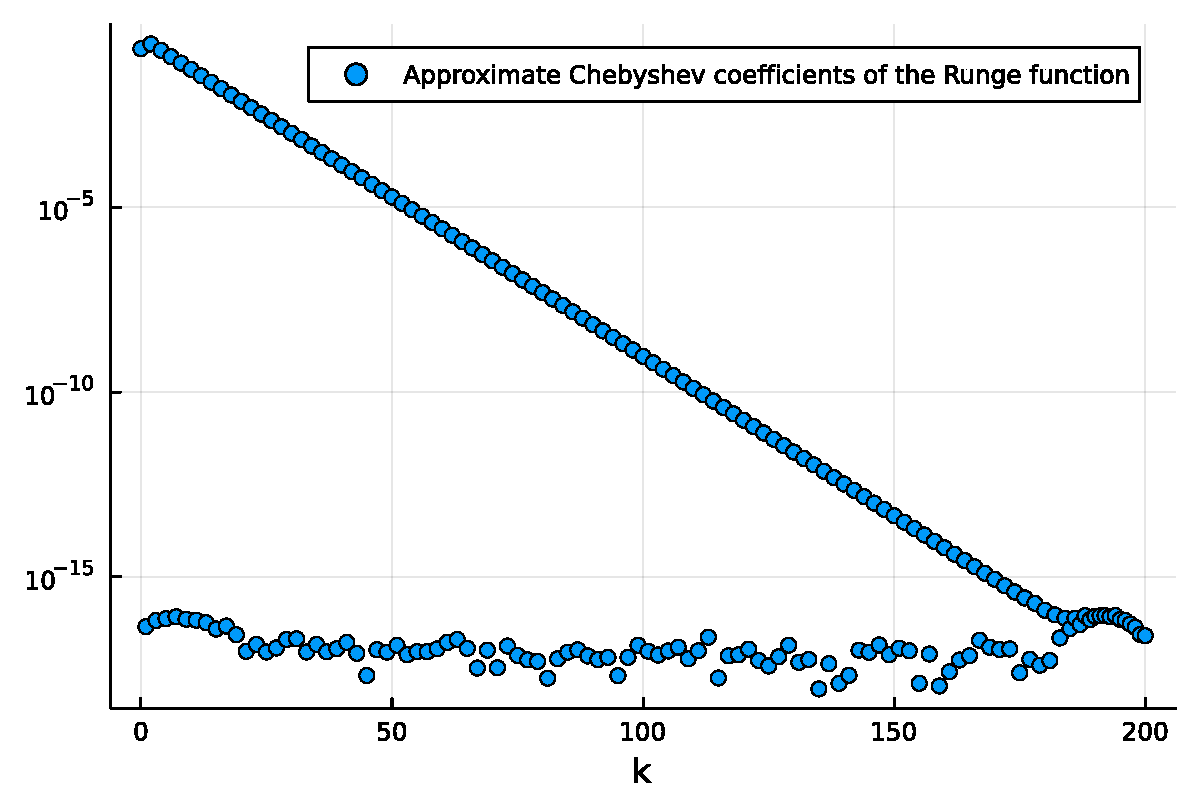
\includegraphics[width=\linewidth]{/figures/Chapter3_6_1.pdf}

The approximate Chebyshev coefficients decay exponentially fast with $k$ because $f(x)$, the Runge function, is analytic on $[-1, 1]$.


\begin{lstlisting}
(*@\HLJLcs{{\#}}@*) (*@\HLJLcs{Map}@*) (*@\HLJLcs{approximate}@*) (*@\HLJLcs{Chebyshev}@*) (*@\HLJLcs{coefficients}@*) (*@\HLJLcs{to}@*) (*@\HLJLcs{function}@*) (*@\HLJLcs{values}@*)
(*@\HLJLnf{norm}@*)(*@\HLJLp{((}@*)(*@\HLJLni{2}@*)(*@\HLJLn{n}@*)(*@\HLJLoB{+}@*)(*@\HLJLni{1}@*)(*@\HLJLp{)}@*)(*@\HLJLoB{*}@*)(*@\HLJLnf{ifft}@*)(*@\HLJLp{(}@*)(*@\HLJLn{ct}@*)(*@\HLJLp{)}@*) (*@\HLJLoB{-}@*) (*@\HLJLn{f}@*)(*@\HLJLoB{.}@*)(*@\HLJLp{(}@*)(*@\HLJLn{cos}@*)(*@\HLJLoB{.}@*)(*@\HLJLp{(}@*)(*@\HLJLn{\ensuremath{\theta}}@*)(*@\HLJLp{)),}@*)(*@\HLJLn{Inf}@*)(*@\HLJLp{)}@*)
\end{lstlisting}

\begin{lstlisting}
3.544325313357017e-16
\end{lstlisting}


In ApproxFun.jl, the command \texttt{Fun(f)} approximates a function using a Chebyshev interpolant (in Chebfun, the command \texttt{chebfun} does the same).  The number of Chebyshev coefficients required the approximate the function to roughly $10^{-16}$ relative accuracy is determined automatically. Here's an example:


\begin{lstlisting}
(*@\HLJLn{fc}@*) (*@\HLJLoB{=}@*) (*@\HLJLnf{Fun}@*)(*@\HLJLp{(}@*)(*@\HLJLn{f}@*)(*@\HLJLp{)}@*)
\end{lstlisting}

\begin{lstlisting}
Fun(Chebyshev(),[0.19611613513818404, 0.0, -0.26361085189847744, 0.0, 0.177
16716982434333, 0.0, -0.11907023492210417, 0.0, 0.0800245376074016, 0.0  (*@\ensuremath{\ldots}@*) 
 0.0, 1.2368591486255537e-16, 0.0, -7.257531816796535e-17, 0.0, 5.855258184
7052e-17, 0.0, -3.05491432152328e-17, 0.0, 2.7525712049567778e-17])
\end{lstlisting}


\begin{lstlisting}
(*@\HLJLnf{length}@*)(*@\HLJLp{(}@*)(*@\HLJLn{fc}@*)(*@\HLJLoB{.}@*)(*@\HLJLn{coefficients}@*)(*@\HLJLp{)}@*)
\end{lstlisting}

\begin{lstlisting}
189
\end{lstlisting}


Let's check that the approximate Chebyshev coefficients we computed with the FFT are approximate equal to the Chebyshev coefficients computed in with ApproxFun:


\begin{lstlisting}
(*@\HLJLnd{@show}@*) (*@\HLJLn{bt}@*)(*@\HLJLp{[}@*)(*@\HLJLni{1}@*)(*@\HLJLoB{:}@*)(*@\HLJLni{189}@*)(*@\HLJLp{]}@*) (*@\HLJLoB{\ensuremath{\approx}}@*) (*@\HLJLn{fc}@*)(*@\HLJLoB{.}@*)(*@\HLJLn{coefficients}@*)
(*@\HLJLnf{norm}@*)(*@\HLJLp{(}@*)(*@\HLJLn{bt}@*)(*@\HLJLp{[}@*)(*@\HLJLni{1}@*)(*@\HLJLoB{:}@*)(*@\HLJLni{189}@*)(*@\HLJLp{]}@*) (*@\HLJLoB{-}@*) (*@\HLJLn{fc}@*)(*@\HLJLoB{.}@*)(*@\HLJLn{coefficients}@*)(*@\HLJLp{,}@*)(*@\HLJLn{Inf}@*)(*@\HLJLp{)}@*)
\end{lstlisting}

\begin{lstlisting}
bt[1:189] (*@\ensuremath{\approx}@*) fc.coefficients = true
1.3121635288093246e-16
\end{lstlisting}


\subsection{Differentiating Chebyshev interpolants with the FFT}
We can approximate derivatives of $f(x)$ by differentiating $q_n(\theta)$ in Fourier coefficient space via the FFT, which is very efficient, as we learnt in Chapter 2. The first derivatives of $p_{n+1}(x)$ and $q_{2n+1}(\theta)$ are related as follows:

\[
f'(x) \approx \frac{{\rm d}}{{\rm d}x}p_{n+1}(x) = \frac{{\rm d}}{{\rm d}x}q_{2n+1}(\theta) = q_{2n+1}'(\theta)\frac{{\rm d} \theta}{\mathrm{d}x} = -\frac{q_{2n+1}'(\theta)}{\sin \theta}
\]

\begin{lstlisting}
(*@\HLJLn{df}@*) (*@\HLJLoB{=}@*) (*@\HLJLn{x}@*) (*@\HLJLoB{->}@*) (*@\HLJLoB{-}@*)(*@\HLJLni{50}@*)(*@\HLJLn{x}@*)(*@\HLJLoB{/}@*)(*@\HLJLp{(}@*)(*@\HLJLni{1}@*) (*@\HLJLoB{+}@*) (*@\HLJLni{25}@*)(*@\HLJLn{x}@*)(*@\HLJLoB{{\textasciicircum}}@*)(*@\HLJLni{2}@*)(*@\HLJLp{)}@*)(*@\HLJLoB{{\textasciicircum}}@*)(*@\HLJLni{2}@*) (*@\HLJLcs{{\#}}@*) (*@\HLJLcs{f{\textquotesingle},}@*) (*@\HLJLcs{the}@*) (*@\HLJLcs{derivative}@*) (*@\HLJLcs{of}@*) (*@\HLJLcs{the}@*) (*@\HLJLcs{Runge}@*) (*@\HLJLcs{function}@*)
(*@\HLJLcs{{\#}}@*) (*@\HLJLcs{differentiate}@*) (*@\HLJLcs{q}@*) (*@\HLJLcs{in}@*) (*@\HLJLcs{coeffcient}@*) (*@\HLJLcs{space}@*) (*@\HLJLcs{and}@*) (*@\HLJLcs{map}@*) (*@\HLJLcs{back}@*) (*@\HLJLcs{to}@*) (*@\HLJLcs{function}@*) (*@\HLJLcs{values}@*) (*@\HLJLcs{space}@*)
(*@\HLJLn{dqn}@*) (*@\HLJLoB{=}@*) (*@\HLJLp{(}@*)(*@\HLJLni{2}@*)(*@\HLJLn{n}@*) (*@\HLJLoB{+}@*) (*@\HLJLni{1}@*)(*@\HLJLp{)}@*)(*@\HLJLoB{*}@*)(*@\HLJLnf{ifft}@*)(*@\HLJLp{(}@*) (*@\HLJLn{im}@*)(*@\HLJLoB{*}@*)(*@\HLJLnf{ifftshift}@*)(*@\HLJLp{(}@*)(*@\HLJLoB{-}@*)(*@\HLJLn{n}@*)(*@\HLJLoB{:}@*)(*@\HLJLn{n}@*)(*@\HLJLp{)}@*)(*@\HLJLoB{.*}@*) (*@\HLJLn{ct}@*)(*@\HLJLp{)}@*) 
(*@\HLJLn{dpn}@*) (*@\HLJLoB{=}@*) (*@\HLJLoB{-}@*)(*@\HLJLn{dqn}@*) (*@\HLJLoB{./}@*)(*@\HLJLn{sin}@*)(*@\HLJLoB{.}@*)(*@\HLJLp{(}@*)(*@\HLJLn{\ensuremath{\theta}}@*)(*@\HLJLp{)}@*)  (*@\HLJLcs{{\#}}@*) (*@\HLJLcs{p\ensuremath{\_n}{\textquotesingle},}@*) (*@\HLJLcs{derivative}@*) (*@\HLJLcs{of}@*) (*@\HLJLcs{p\ensuremath{\_n}}@*)
(*@\HLJLn{x}@*) (*@\HLJLoB{=}@*) (*@\HLJLn{cos}@*)(*@\HLJLoB{.}@*)(*@\HLJLp{(}@*)(*@\HLJLn{\ensuremath{\theta}}@*)(*@\HLJLp{)}@*)
(*@\HLJLcs{{\#}}@*) (*@\HLJLcs{the}@*) (*@\HLJLcs{error}@*) (*@\HLJLcs{of}@*) (*@\HLJLcs{the}@*) (*@\HLJLcs{approximation}@*) (*@\HLJLcs{f{\textquotesingle}}@*) (*@\HLJLcs{\ensuremath{\approx}}@*) (*@\HLJLcs{p{\textquotesingle}}@*)
(*@\HLJLnf{norm}@*)(*@\HLJLp{(}@*)(*@\HLJLn{df}@*)(*@\HLJLoB{.}@*)(*@\HLJLp{(}@*)(*@\HLJLn{x}@*)(*@\HLJLp{[}@*)(*@\HLJLni{2}@*)(*@\HLJLoB{:}@*)(*@\HLJLk{end}@*)(*@\HLJLp{])}@*) (*@\HLJLoB{-}@*) (*@\HLJLn{dpn}@*)(*@\HLJLp{[}@*)(*@\HLJLni{2}@*)(*@\HLJLoB{:}@*)(*@\HLJLk{end}@*)(*@\HLJLp{],}@*)(*@\HLJLn{Inf}@*)(*@\HLJLp{)}@*)
\end{lstlisting}

\begin{lstlisting}
1.340491672910366e-12
\end{lstlisting}


Note that $p_{n+1}'(x) = -q_{2n+1}'(\theta)/\sin \theta$ is not well-defined for $\theta = 0, \pi$ (i.e., at $x = \cos\theta =  \pm 1$).  For these cases we use l'Hopital's rule.

We typically prefer to approximate a function (or solution to a differential equation) at the \emph{Chebyshev points}, 

\[
x_j = \cos\left(\frac{j\pi}{n}\right), \qquad j = 0, \ldots, n,
\]
because these include the end points of the interval $[-1, 1]$ where we typically impose boundary conditions.

Here is a function that takes as input the function values $f(x_j)$, $j = 0, \ldots, n$ at the Chebyshev points and it returns $p_{n+1}'(x_j)$, $j = 0, \ldots, n$ via the FFT (i.e., the derivate of the Chebyshev interpolant at the Chebyshev points, which approximate $f'(x_j)$). The formulae for performing differentiation at the Chebyshev points via the FFT are slightly different from the formulae discussed above, where we considered a different set of points, namely $x_j = \cos\theta_j = \cos\left( \frac{2\pi j}{2n + 1}  \right), j = 0, \ldots, 2n$


\begin{lstlisting}
(*@\HLJLk{function}@*) (*@\HLJLnf{chebfft}@*)(*@\HLJLp{(}@*)(*@\HLJLn{f}@*)(*@\HLJLp{)}@*)
    (*@\HLJLn{n}@*) (*@\HLJLoB{=}@*) (*@\HLJLnf{length}@*)(*@\HLJLp{(}@*)(*@\HLJLn{f}@*)(*@\HLJLp{)}@*)(*@\HLJLoB{-}@*)(*@\HLJLni{1}@*)
    (*@\HLJLn{x}@*) (*@\HLJLoB{=}@*) (*@\HLJLn{cos}@*)(*@\HLJLoB{.}@*)(*@\HLJLp{((}@*)(*@\HLJLni{0}@*)(*@\HLJLoB{:}@*)(*@\HLJLn{n}@*)(*@\HLJLp{)}@*)(*@\HLJLoB{*}@*)(*@\HLJLn{\ensuremath{\pi}}@*)(*@\HLJLoB{/}@*)(*@\HLJLn{n}@*)(*@\HLJLp{)}@*) (*@\HLJLcs{{\#}}@*) (*@\HLJLcs{Chebyshev}@*) (*@\HLJLcs{points}@*)
    (*@\HLJLn{ii}@*) (*@\HLJLoB{=}@*) (*@\HLJLni{0}@*)(*@\HLJLoB{:}@*)(*@\HLJLn{n}@*)(*@\HLJLoB{-}@*)(*@\HLJLni{1}@*)
    (*@\HLJLn{q}@*) (*@\HLJLoB{=}@*) (*@\HLJLp{[}@*)(*@\HLJLn{f}@*)(*@\HLJLp{;}@*) (*@\HLJLn{f}@*)(*@\HLJLp{[}@*)(*@\HLJLn{n}@*)(*@\HLJLoB{:-}@*)(*@\HLJLni{1}@*)(*@\HLJLoB{:}@*)(*@\HLJLni{2}@*)(*@\HLJLp{]]}@*)      (*@\HLJLcs{{\#}}@*) (*@\HLJLcs{transform}@*) (*@\HLJLcs{x}@*) (*@\HLJLcs{->}@*) (*@\HLJLcs{\ensuremath{\theta}}@*)    
    (*@\HLJLcs{{\#}}@*) (*@\HLJLcs{differentiate}@*) (*@\HLJLcs{the}@*) (*@\HLJLcs{interpolant}@*) (*@\HLJLcs{q\ensuremath{\_n}}@*) (*@\HLJLcs{in}@*) (*@\HLJLcs{coefficient}@*) (*@\HLJLcs{space}@*) (*@\HLJLcs{and}@*) (*@\HLJLcs{map}@*) (*@\HLJLcs{back}@*) (*@\HLJLcs{to}@*) (*@\HLJLcs{function}@*) (*@\HLJLcs{values}@*)
    (*@\HLJLn{cq}@*) (*@\HLJLoB{=}@*) (*@\HLJLn{real}@*)(*@\HLJLoB{.}@*)(*@\HLJLp{(}@*)(*@\HLJLnf{fft}@*)(*@\HLJLp{(}@*)(*@\HLJLn{q}@*)(*@\HLJLp{))}@*)
    (*@\HLJLn{dq}@*) (*@\HLJLoB{=}@*) (*@\HLJLn{real}@*)(*@\HLJLoB{.}@*)(*@\HLJLp{(}@*)(*@\HLJLnf{ifft}@*)(*@\HLJLp{(}@*)(*@\HLJLn{im}@*)(*@\HLJLoB{*}@*)(*@\HLJLp{[}@*)(*@\HLJLn{ii}@*)(*@\HLJLp{;}@*) (*@\HLJLni{0}@*)(*@\HLJLp{;}@*) (*@\HLJLni{1}@*)(*@\HLJLoB{-}@*)(*@\HLJLn{n}@*)(*@\HLJLoB{:-}@*)(*@\HLJLni{1}@*)(*@\HLJLp{]}@*) (*@\HLJLoB{.*}@*)(*@\HLJLn{cq}@*)(*@\HLJLp{))}@*)
    (*@\HLJLn{df}@*) (*@\HLJLoB{=}@*) (*@\HLJLnf{zeros}@*)(*@\HLJLp{(}@*)(*@\HLJLn{n}@*)(*@\HLJLoB{+}@*)(*@\HLJLni{1}@*)(*@\HLJLp{,}@*)(*@\HLJLni{1}@*)(*@\HLJLp{)}@*)
    (*@\HLJLcs{{\#}}@*) (*@\HLJLcs{Compute}@*) (*@\HLJLcs{approximations}@*) (*@\HLJLcs{to}@*) (*@\HLJLcs{f{\textquotesingle}}@*) (*@\HLJLcs{at}@*) (*@\HLJLcs{the}@*) (*@\HLJLcs{interior}@*) (*@\HLJLcs{points}@*)
    (*@\HLJLn{df}@*)(*@\HLJLp{[}@*)(*@\HLJLni{2}@*)(*@\HLJLoB{:}@*)(*@\HLJLn{n}@*)(*@\HLJLp{]}@*) (*@\HLJLoB{=}@*) (*@\HLJLoB{-}@*)(*@\HLJLn{dq}@*)(*@\HLJLp{[}@*)(*@\HLJLni{2}@*)(*@\HLJLoB{:}@*)(*@\HLJLn{n}@*)(*@\HLJLp{]}@*) (*@\HLJLoB{./}@*)(*@\HLJLn{sqrt}@*)(*@\HLJLoB{.}@*)(*@\HLJLp{(}@*)(*@\HLJLni{1}@*) (*@\HLJLoB{.-}@*) (*@\HLJLn{x}@*)(*@\HLJLp{[}@*)(*@\HLJLni{2}@*)(*@\HLJLoB{:}@*)(*@\HLJLn{n}@*)(*@\HLJLp{]}@*)(*@\HLJLoB{.{\textasciicircum}}@*)(*@\HLJLni{2}@*)(*@\HLJLp{)}@*)    (*@\HLJLcs{{\#}}@*) (*@\HLJLcs{transform}@*) (*@\HLJLcs{\ensuremath{\theta}}@*) (*@\HLJLcs{->}@*) (*@\HLJLcs{x}@*)   
    (*@\HLJLcs{{\#}}@*) (*@\HLJLcs{At}@*) (*@\HLJLcs{the}@*) (*@\HLJLcs{boundary}@*) (*@\HLJLcs{points}@*)
    (*@\HLJLn{df}@*)(*@\HLJLp{[}@*)(*@\HLJLni{1}@*)(*@\HLJLp{]}@*) (*@\HLJLoB{=}@*) (*@\HLJLnf{sum}@*)(*@\HLJLp{(}@*)(*@\HLJLn{ii}@*)(*@\HLJLoB{.{\textasciicircum}}@*)(*@\HLJLni{2}@*) (*@\HLJLoB{.*}@*)(*@\HLJLn{cq}@*)(*@\HLJLp{[}@*)(*@\HLJLni{1}@*)(*@\HLJLoB{:}@*)(*@\HLJLn{n}@*)(*@\HLJLp{])}@*)(*@\HLJLoB{/}@*)(*@\HLJLn{n}@*) (*@\HLJLoB{+}@*) (*@\HLJLnfB{.5}@*)(*@\HLJLoB{*}@*)(*@\HLJLn{n}@*)(*@\HLJLoB{*}@*)(*@\HLJLn{cq}@*)(*@\HLJLp{[}@*)(*@\HLJLn{n}@*)(*@\HLJLoB{+}@*)(*@\HLJLni{1}@*)(*@\HLJLp{]}@*)     
    (*@\HLJLn{df}@*)(*@\HLJLp{[}@*)(*@\HLJLn{n}@*)(*@\HLJLoB{+}@*)(*@\HLJLni{1}@*)(*@\HLJLp{]}@*) (*@\HLJLoB{=}@*) (*@\HLJLnf{sum}@*)(*@\HLJLp{((}@*)(*@\HLJLoB{-}@*)(*@\HLJLni{1}@*)(*@\HLJLp{)}@*) (*@\HLJLoB{.{\textasciicircum}}@*)(*@\HLJLp{(}@*)(*@\HLJLn{ii}@*) (*@\HLJLoB{.+}@*)(*@\HLJLni{1}@*)(*@\HLJLp{)}@*) (*@\HLJLoB{.*}@*) (*@\HLJLn{ii}@*)(*@\HLJLoB{.{\textasciicircum}}@*)(*@\HLJLni{2}@*) (*@\HLJLoB{.*}@*)(*@\HLJLn{cq}@*)(*@\HLJLp{[}@*)(*@\HLJLni{1}@*)(*@\HLJLoB{:}@*)(*@\HLJLn{n}@*)(*@\HLJLp{])}@*)(*@\HLJLoB{/}@*)(*@\HLJLn{n}@*) (*@\HLJLoB{+}@*)
              (*@\HLJLnfB{.5}@*)(*@\HLJLoB{*}@*)(*@\HLJLp{(}@*)(*@\HLJLoB{-}@*)(*@\HLJLni{1}@*)(*@\HLJLp{)}@*)(*@\HLJLoB{{\textasciicircum}}@*)(*@\HLJLp{(}@*)(*@\HLJLn{n}@*)(*@\HLJLoB{+}@*)(*@\HLJLni{1}@*)(*@\HLJLp{)}@*)(*@\HLJLoB{*}@*)(*@\HLJLn{n}@*)(*@\HLJLoB{*}@*)(*@\HLJLn{cq}@*)(*@\HLJLp{[}@*)(*@\HLJLn{n}@*)(*@\HLJLoB{+}@*)(*@\HLJLni{1}@*)(*@\HLJLp{]}@*)
    (*@\HLJLn{df}@*)
(*@\HLJLk{end}@*)
\end{lstlisting}

\begin{lstlisting}
chebfft (generic function with 1 method)
\end{lstlisting}


Let's test \texttt{chebfft}:


\begin{lstlisting}
(*@\HLJLn{x}@*) (*@\HLJLoB{=}@*) (*@\HLJLn{cos}@*)(*@\HLJLoB{.}@*)(*@\HLJLp{((}@*)(*@\HLJLni{0}@*)(*@\HLJLoB{:}@*)(*@\HLJLn{n}@*)(*@\HLJLp{)}@*)(*@\HLJLoB{*}@*)(*@\HLJLn{\ensuremath{\pi}}@*)(*@\HLJLoB{/}@*)(*@\HLJLn{n}@*)(*@\HLJLp{)}@*)
(*@\HLJLnf{norm}@*)(*@\HLJLp{(}@*)(*@\HLJLnf{chebfft}@*)(*@\HLJLp{(}@*)(*@\HLJLn{f}@*)(*@\HLJLoB{.}@*)(*@\HLJLp{(}@*)(*@\HLJLn{x}@*)(*@\HLJLp{))}@*) (*@\HLJLoB{-}@*) (*@\HLJLn{df}@*)(*@\HLJLoB{.}@*)(*@\HLJLp{(}@*)(*@\HLJLn{x}@*)(*@\HLJLp{),}@*)(*@\HLJLn{Inf}@*)(*@\HLJLp{)}@*)
\end{lstlisting}

\begin{lstlisting}
1.562694418311139e-12
\end{lstlisting}


\subsection{Differentiation matrices for Chebyshev interpolants}
In Chapter 2 we learnt about two equivalent representations of the trigonometric interpolant ("coefficient space" and "value space"), each expressed in terms of different basis functions.  Here we do the same for polynomial interpolants in the Chebyshev points. We have already seen one representation as an expansion in Chebyshev polynomials and approximate Chebyshev coefficients,

\[
p_{n+1}(x) = \sum_{k = 0}^{n}\tilde{b}_k^n T_k(x),
\]
which allowed us to leverage Fourier series to compute $\tilde{b}_k^n$ and derivatives of $p_{n+1}(x)$ via the FFT.  We now build differentiation matrices that act on function values to compute derivatives of $p_{n+1}(x)$ by using its representation in terms of Lagrange basis polynomials and function values.

Recall from the formula for the Lagrange interpolating polynomial that

\[
p_{n+1}(x) = \sum_{k = 0}^{n}\ell_k(x)f(x_k), \qquad \ell_k(x) = \prod_{\substack{j=0\\ j \neq k}}^{k}\frac{x-x_j}{x_k-x_j}
\]
here we let $x_k$ be the Chebyshev points 

\[
x_k = \cos\left(\frac{\pi k}{n} \right), \qquad k = 0, \ldots, n.
\]
We can represent differentiation of the Chebyshev interpolant via an $(n+1) \times (n+1)$ differentiation matrix $D_n$: since

\[
p_{n+1}'(x) = \sum_{k = 0}^{n}\ell_k'(x)f(x_k),
\]
we have

\[
\begin{bmatrix}
p_{n+1}'(x_0) \\
\vdots \\
p_{n+1}'(x_n)
\end{bmatrix} = 
\begin{bmatrix}
\ell_0'(x_0) & \cdots & \ell_n'(x_0) \\
\vdots & \vdots  & \vdots \\
\ell_0'(x_n) & \cdots & \ell_n'(x_n)
\end{bmatrix}
\begin{bmatrix}
f(x_0) \\
\vdots \\
f(x_n)
\end{bmatrix}
\]
or in vector form,

\[
\mathbf{p}' = D_n \mathbf{f}.
\]
Here is a function that builds the differentiation matrix $D_n$:


\begin{lstlisting}
(*@\HLJLk{function}@*) (*@\HLJLnf{cheb}@*)(*@\HLJLp{(}@*)(*@\HLJLn{n}@*)(*@\HLJLp{)}@*)

    (*@\HLJLn{x}@*) (*@\HLJLoB{=}@*) (*@\HLJLn{cos}@*)(*@\HLJLoB{.}@*)(*@\HLJLp{(}@*)(*@\HLJLn{\ensuremath{\pi}}@*)(*@\HLJLoB{*}@*)(*@\HLJLp{(}@*)(*@\HLJLni{0}@*)(*@\HLJLoB{:}@*)(*@\HLJLn{n}@*)(*@\HLJLp{)}@*)(*@\HLJLoB{/}@*)(*@\HLJLn{n}@*)(*@\HLJLp{)}@*)
    (*@\HLJLn{c}@*) (*@\HLJLoB{=}@*) (*@\HLJLp{[}@*)(*@\HLJLni{2}@*)(*@\HLJLp{;}@*) (*@\HLJLnf{ones}@*)(*@\HLJLp{(}@*)(*@\HLJLn{n}@*)(*@\HLJLoB{-}@*)(*@\HLJLni{1}@*)(*@\HLJLp{,}@*)(*@\HLJLni{1}@*)(*@\HLJLp{);}@*) (*@\HLJLni{2}@*)(*@\HLJLp{]}@*)(*@\HLJLoB{.*}@*)(*@\HLJLp{(}@*)(*@\HLJLoB{-}@*)(*@\HLJLni{1}@*)(*@\HLJLp{)}@*)(*@\HLJLoB{.{\textasciicircum}}@*)(*@\HLJLp{(}@*)(*@\HLJLni{0}@*)(*@\HLJLoB{:}@*)(*@\HLJLn{n}@*)(*@\HLJLp{)}@*)
    (*@\HLJLn{X}@*) (*@\HLJLoB{=}@*) (*@\HLJLnf{repeat}@*)(*@\HLJLp{(}@*)(*@\HLJLn{x}@*)(*@\HLJLp{,}@*)(*@\HLJLni{1}@*)(*@\HLJLp{,}@*)(*@\HLJLn{n}@*)(*@\HLJLoB{+}@*)(*@\HLJLni{1}@*)(*@\HLJLp{)}@*)
    (*@\HLJLn{dX}@*) (*@\HLJLoB{=}@*) (*@\HLJLn{X}@*)(*@\HLJLoB{-}@*)(*@\HLJLn{X}@*)(*@\HLJLoB{{\textquotesingle}}@*)
    (*@\HLJLn{D}@*) (*@\HLJLoB{=}@*) (*@\HLJLp{(}@*)(*@\HLJLn{c}@*)(*@\HLJLoB{*}@*)(*@\HLJLp{(}@*)(*@\HLJLni{1}@*) (*@\HLJLoB{./}@*)(*@\HLJLn{c}@*)(*@\HLJLp{)}@*)(*@\HLJLoB{{\textquotesingle}}@*)(*@\HLJLp{)}@*)(*@\HLJLoB{./}@*)(*@\HLJLp{(}@*) (*@\HLJLn{dX}@*) (*@\HLJLoB{+}@*) (*@\HLJLn{I}@*) (*@\HLJLp{)}@*) (*@\HLJLcs{{\#}}@*) (*@\HLJLcs{off-diagonal}@*) (*@\HLJLcs{entries}@*)
    (*@\HLJLn{D}@*) (*@\HLJLoB{=}@*) (*@\HLJLn{D}@*) (*@\HLJLoB{-}@*) (*@\HLJLnf{diagm}@*)(*@\HLJLp{(}@*)(*@\HLJLnf{vec}@*)(*@\HLJLp{(}@*)(*@\HLJLnf{sum}@*)(*@\HLJLp{(}@*)(*@\HLJLn{D}@*)(*@\HLJLoB{{\textquotesingle}}@*)(*@\HLJLp{;}@*)(*@\HLJLn{dims}@*)(*@\HLJLoB{=}@*)(*@\HLJLni{1}@*)(*@\HLJLp{)))}@*)(*@\HLJLcs{{\#}}@*) (*@\HLJLcs{diagonal}@*) (*@\HLJLcs{entries}@*)
    
    (*@\HLJLn{D}@*)(*@\HLJLp{,}@*) (*@\HLJLn{x}@*)

(*@\HLJLk{end}@*)
\end{lstlisting}

\begin{lstlisting}
cheb (generic function with 1 method)
\end{lstlisting}


To summarise, we have two equivalent methods for computing the derivate of the Chebyshev interpolant at the $n+1$ Chebyshev points.  The FFT method has $\mathcal{O}(n\log n)$ complexity while  applying a differentiation matrix to a vector requires $\mathcal{O}(n^2)$ operations because $D_n$ is a dense matrix.

Let's check that the two methods give the same output (up to rounding errors):


\begin{lstlisting}
(*@\HLJLn{n}@*) (*@\HLJLoB{=}@*) (*@\HLJLni{50}@*)
(*@\HLJLn{D}@*)(*@\HLJLp{,}@*)(*@\HLJLn{x}@*) (*@\HLJLoB{=}@*) (*@\HLJLnf{cheb}@*)(*@\HLJLp{(}@*)(*@\HLJLn{n}@*)(*@\HLJLp{)}@*)
(*@\HLJLnd{@show}@*) (*@\HLJLn{D}@*)(*@\HLJLoB{*}@*)(*@\HLJLn{f}@*)(*@\HLJLoB{.}@*)(*@\HLJLp{(}@*)(*@\HLJLn{x}@*)(*@\HLJLp{)}@*) (*@\HLJLoB{\ensuremath{\approx}}@*) (*@\HLJLnf{chebfft}@*)(*@\HLJLp{(}@*)(*@\HLJLn{f}@*)(*@\HLJLoB{.}@*)(*@\HLJLp{(}@*)(*@\HLJLn{x}@*)(*@\HLJLp{))}@*)
(*@\HLJLnf{norm}@*)(*@\HLJLp{(}@*)(*@\HLJLn{D}@*)(*@\HLJLoB{*}@*)(*@\HLJLn{f}@*)(*@\HLJLoB{.}@*)(*@\HLJLp{(}@*)(*@\HLJLn{x}@*)(*@\HLJLp{)}@*) (*@\HLJLoB{-}@*) (*@\HLJLnf{chebfft}@*)(*@\HLJLp{(}@*)(*@\HLJLn{f}@*)(*@\HLJLoB{.}@*)(*@\HLJLp{(}@*)(*@\HLJLn{x}@*)(*@\HLJLp{)),}@*)(*@\HLJLn{Inf}@*)(*@\HLJLp{)}@*)
\end{lstlisting}

\begin{lstlisting}
D * f.(x) (*@\ensuremath{\approx}@*) chebfft(f.(x)) = true
6.061817714453355e-14
\end{lstlisting}


\subsection{A PDE example: the wave equation}
Consider the following $(1+1)$-dimensional wave equation PDE initial / boundary value problem 

\[
u_{tt} = u_{xx}, \qquad t > 0, \qquad -1 < x < 1, \qquad u(\pm 1, t) = 0,
\]
subject to the initial data

\[
u(x,0) = f(x), \qquad u_t(x,0) = g(x), \qquad x \in [-1, 1],
\]
where we assume that $f$ and $g$ are not both identically zero (because then the trivial solution $u(x,t) = 0$ solves the problem).  We are going to approximate the solution to this problem by approximating $u_{tt}$ with finite differences and $u_{xx}$ with differentiation of a Chebyshev interpolant in $x$. First, we derive the exact solution to this problem using the method of separation of variables. 

\subsubsection{The method of separation of variables}
We attempt to find a solution of the form

\[
u(x,t) = X(x)T(t).
\]
From the zero boundary conditions, we conclude that

\[
u(-1,t) = X(-1)T(t) = 0 = T(t)X(1) = u(1,t) \quad \Rightarrow \quad X(-1) = 0 = X(1).
\]
Substituting $u = XT$  into the PDE, we find that

\[
\frac{T''(t)}{T(t)} = \frac{X''(x)}{X(x)}. 
\]
This can hold only if 

\[
\frac{T''(t)}{T(t)} = \frac{X''(x)}{X(x)} = \lambda \in \mathbb{R}.
\]
We need to consider three cases

\begin{itemize}
\item[1. ] \[
\lambda > 0
\]

\item[2. ] \[
\lambda = 0
\]

\item[3. ] \[
\lambda < 0
\]
\end{itemize}
Cases (1) and (2) are left as an exercise. 

For case (3), we set $\lambda = - \kappa^2$ with $\kappa \in \mathbb{R}\setminus \{0\}$ then for $X$ we have the ODE boundary-value (or eigenvalue) problem

\[
X'' = -\kappa^2 X, \qquad X(-1) = 0 = X(1)
\]
The general solution to the ODE $X''+\kappa^2 X = 0$ is $X = c_1 \sin\kappa x + c_2\cos\kappa x$, for arbitrary constants $c_1$, $c_2$ ($\sin\kappa x$ and $\cos\kappa x$ are eigenfunctions of the differential operator $\frac{{\rm d}^2}{{\rm d}x^2}$). To satisfy the boundary conditions $X(-1) = 0 = X(1)$, we require

\[
-c_1 \sin\kappa + c_2\cos\kappa = 0 = c_1 \sin\kappa  + c_2\cos\kappa .
\]
Since $\kappa \neq 0$ and $\sin \kappa$ and $\cos \kappa$ are linearly independent functions, these equations hold only if $c_1 = c_2 = 0$, which implies that $X=0$ which would give the inadmissable solution $u = 0$.  Instead, we attempt to find solutions of the form (i) $X = c_1 \sin\kappa x$  and (ii) $X = c_1 \cos\kappa x$.  For case (i), we require

\[
    \kappa = \kappa_n = \pi n, \qquad n \neq 0,
\]
in order to satisfy $X(-1) = 0 = X(1)$ and for case (ii),

\[
\kappa = \kappa_n = (2n + 1)\frac{\pi}{2}
\]
where $n \in \mathbb{Z}$.  For case (i), $T$ has the solution

\[
T(t) = c_1 \sin\kappa_n t + c_2\cos\kappa_n t   \qquad (1)
\]
with $\kappa_n = \pi n$ and in case (ii), $T$ has the solution (1) with $\kappa_n = (2n + 1)\frac{\pi}{2}$.  As before, $c_1$ and $c_2$ are arbitrary constants.  We have therefore constructed two families of solutions to the wave equation:

\[
u = \left( c_1 \sin\kappa_n t + c_2\cos\kappa_n t \right)\sin \kappa_n x, \qquad \kappa_n = \pi n
\]
and

\[
u = \left( b_1 \sin\kappa_n t + b_2\cos\kappa_n t \right)\cos \kappa_n x, \qquad \kappa_n =(2n + 1)\frac{\pi}{2}.
\]
Since the wave equation is linear, any scalar multiples and linear combinations of the solutions above are also solutions to the PDE initial / boundary-value problem. 

Therfore the following series is a formal solution to the PDE,

\[
u(x,t) = \sum_{n = 1}^{\infty} \left(\alpha_n\sin\pi n t + \beta_n\cos\pi n t  \right)\sin\pi n x +  \sum_{n = 0}^{\infty} \left(\gamma_n\sin \kappa_n t + \delta_n\cos \kappa_n t  \right)\cos\kappa_n x,
\]
where $\kappa_n =(2n + 1)\frac{\pi}{2}$ and  $\alpha_n, \beta_n, \gamma_n, \delta_n$ are arbitrary constants whose values we shall determine by using the initial data:

\[
u(x,0) = \sum_{n = 1}^{\infty} \beta_n  \sin\pi n x +  \sum_{n = 0}^{\infty} \delta_n \cos\kappa_n x = f(x)
\]
\[
u_t(x,0) = \sum_{n = 1}^{\infty} \pi n\alpha_n  \sin\pi n x +  \sum_{n = 0}^{\infty}\kappa_n \gamma_n \cos\kappa_n x = g(x)
\]
Using the fact that 

\[
\int_{-1}^{1} \sin \pi n x \sin \pi m x\, {\rm d}x = \delta_{n,m} = \begin{cases}
1 & \text{if } n = m \\
0 & \text{otherwise}
\end{cases}
\]
\[
\int_{-1}^{1} \sin \pi n x \cos \kappa_m x\, {\rm d}x = 0, \qquad n, m \geq 0 
\]
and

\[
\int_{-1}^{1} \cos \kappa_n x \cos \kappa_m x\, {\rm d}x = \delta_{n,m} 
\]
it follows that

\[
\beta_m = \int_{-1}^{1} f(x) \sin m\pi x \,{\rm d}x, \quad m\geq 1, \qquad \delta_m = \int_{-1}^{1} f(x) \cos \kappa_m x \,{\rm d}x,\quad m \geq 0
\]
and

\[
\alpha_m = \frac{1}{\pi n}\int_{-1}^{1} g(x) \sin m\pi x \,{\rm d}x, \quad m\geq 1, \qquad \gamma_m = \frac{1}{\kappa_n}\int_{-1}^{1} g(x) \cos \kappa_m x \,{\rm d}x,\quad m \geq 0.
\]
We have derived the exact solution to the PDE intial/boundary value problem as the sum of two series: a sine series (in $x$) and a cosine series (in $x$), each with time-dependent coefficients that are themselves expressed in terms of trigonometric functions.  We can express the sine and cosine series as Fourier series with time-dependent coefficients.  To compute an approximation to the solution, we could use the FFT to compute approximate coefficients  $\tilde{\alpha}_n$, $\tilde{\beta}_n$, $\tilde{\gamma}_n$, $\tilde{\delta}_n$ and then set

\[
u(x,t) \approx \sum_{n = 1}^{N} \left(\tilde{\alpha}_n\sin\pi n t + \tilde{\beta}_n\cos\pi n t  \right)\sin\pi n x +  \sum_{n = 0}^{N} \left(\tilde{\gamma}_n\sin \kappa_n t + \tilde{\delta}_n\cos \kappa_n t  \right)\cos\kappa_n x.
\]
This method relies on knowing the exact solution to the problem, which may not be possible for a more complicated PDE. Instead, we shall compute an approximate solution using a combination of finite differences and Chebyshev interpolants, which is a method which doesn't require knowing the exact solution.

\textbf{Remark} We derived an exact solution to the initial / boundary-value PDE problem above.  If we consider the "pure" initial-value problem (the Cauchy problem) for the wave equation on the whole real line, i.e., 

\[
u_{tt} = u_{xx}, \qquad t > 0, \qquad x \in \mathbb{R},
\]
note there are no boundary conditions, then it is easy to verify that 

\[
u(x,t) = F(x-t) + G(x+t)
\]
is a solution to the Cauchy problem, where $F$ and $G$ are unknown functions that can be determined from the initial data

\[
u(x,0) = f(x), \qquad u_t(x,0) = g(x).
\]
This solution can be derived using the method of characteristics. 

\subsubsection{Numerical solution}
We consider the initial / boundary-value problem for the wave equation

\[
u_{tt} = u_{xx}, \qquad t > 0, \qquad -1 < x < 1, \qquad u(\pm 1, t) = 0.
\]
We discretise $x$ using the Chebyshev points,

\[
x_j =  \cos\left(  \frac{j\pi}{n_x}\right), \qquad j = 0, \ldots, n_x, 
\]
and we let $t \in [0, T]$ and set

\[
t_i = i\tau, \qquad \tau = \frac{T}{n_t}, \qquad i = 0, \ldots, n_t.
\]
We let $u^{i}_j$ denote the approximation to the exact solution $u$ at $x=x_j$ and $t = t_i$, i.e.,

\[
u^{i}_j \approx u(x_j, t_i),
\]
and we let $\mathbf{u}^{i}$ denote the vector of approximations at "time-level" $i$:

\[
\mathbf{u}^{i} = \begin{bmatrix}
u^{i}_0 \\
u^{i}_1 \\
\vdots \\
u^{i}_n
\end{bmatrix}.
\]
The second time-derivative is approximated with a central difference approximation (see Chapter 1, Exercise 1):

\[
u_{tt}(x_j,t_i) \approx \frac{u(x_j,t_{i+1}) - 2u(x_j,t_{i}) + u(x_j,t_{i-1})}{\tau^2} \approx \frac{u^{i+1}_j - 2u^{i}_j + u^{i-1}_j}{\tau^2}, \qquad j = 0, \ldots, n_x
\]
or, in vector notation,

\[
u_{tt}(\mathbf{x},t_i) \approx \frac{\mathbf{u}^{i+1} - 2\mathbf{u}^{i} + \mathbf{u}^{i-1}}{\tau^2}.
\]
The spatial derivative is approximated by differentiation of a Chebyshev interpolant in $x$: 

\[
\begin{bmatrix}
u_x(x_0,t_i) \\
\vdots \\
u_x(x_n,t_i)
\end{bmatrix} \approx 
\begin{bmatrix}
\ell_0'(x_0) & \cdots & \ell_n'(x_0) \\
\vdots & \vdots  & \vdots \\
\ell_0'(x_n) & \cdots & \ell_n'(x_n)
\end{bmatrix}
\begin{bmatrix}
u(x_0,t_i) \\
\vdots \\
u(x_n,t_i) 
\end{bmatrix}
\approx
\begin{bmatrix}
\ell_0'(x_0) & \cdots & \ell_n'(x_0) \\
\vdots & \vdots  & \vdots \\
\ell_0'(x_n) & \cdots & \ell_n'(x_n)
\end{bmatrix}
\begin{bmatrix}
u_0^i \\
\vdots \\
u_n^i
\end{bmatrix}
\]
i.e.,

\[
u_{x}(\mathbf{x},t_i) \approx D_n\mathbf{u}^{i}
\]
and

\[
u_{xx}(\mathbf{x},t_i) \approx D_n\left(D_n\mathbf{u}^{i}\right) = D_n^2\mathbf{u}^{i}.
\]
Therefore we approximate the solution to the PDE as follows:

\[
\mathbf{u}^{i+1} = 2\mathbf{u}^{i} - \mathbf{u}^{i-1} + \tau^2 D_n^2\mathbf{u}^{i}, \qquad i = 0, \ldots, n_t-1.
\]
\textbf{Remark} Note that we don't need to include the approximations $u_0^{i}$ and $u_n^{i}$ since we know the solution values at $x = \pm 1$ from the zero boundary conditions $u(\pm 1, t) = 0$.  For now we ignore this fact since we shall discuss the imposition of boundary conditions later in this module.

\textbf{Remark} In practice, we don't compute $D_n^2\mathbf{u}^{i}$ by building the differentiation matrix $D_n$ and squaring it, since it costs $\mathcal{O}(n_x^3)$ operations, however computing $D_n(D_n\mathbf{u}^{i})$ has $\mathcal{O}(n_x^2)$ complexity. As we showed above, $D_n\mathbf{u}^{i}$ can be computed with the FFT with $\mathcal{O}(n_x\log n_x)$ complexity, so we compute $D_n^2\mathbf{u}^{i}$ by differentiating twice via the FFT, which thus also has $\mathcal{O}(n_x\log n_x)$ complexity.

We require two starting values to implement the numerical method.  We let

\[
u(x,0) = f(x) = {\rm e}^{-200x^2}.
\]
Rather than specifying $u_t(x,0)$, we impose the condition

\[
u(x,-\tau) = f(x - \tau) = {\rm e}^{-200(x-\tau)^2}.
\]
(Recall that $u(x,t) = F(x+t)$ is a solution to the Cauchy problem for the wave equation).  Hence, the numerical method is 

\[
\mathbf{u}^{0} = f(\mathbf{x}), \qquad \mathbf{u}^{-1} = f(\mathbf{x}-\tau), \qquad \mathbf{u}^{i+1} = 2\mathbf{u}^{i} - \mathbf{u}^{i-1} + \tau^2 D_n^2\mathbf{u}^{i}, \qquad i = 0, \ldots, n_t-1.
\]

\begin{lstlisting}
(*@\HLJLn{N}@*) (*@\HLJLoB{=}@*) (*@\HLJLni{80}@*)(*@\HLJLp{;}@*) (*@\HLJLn{x}@*) (*@\HLJLoB{=}@*) (*@\HLJLn{cos}@*)(*@\HLJLoB{.}@*)(*@\HLJLp{(}@*)(*@\HLJLn{\ensuremath{\pi}}@*)(*@\HLJLoB{*}@*)(*@\HLJLp{(}@*)(*@\HLJLni{0}@*)(*@\HLJLoB{:}@*)(*@\HLJLn{N}@*)(*@\HLJLp{)}@*)(*@\HLJLoB{/}@*)(*@\HLJLn{N}@*)(*@\HLJLp{);}@*) (*@\HLJLn{dt}@*) (*@\HLJLoB{=}@*) (*@\HLJLni{8}@*)(*@\HLJLoB{/}@*)(*@\HLJLn{N}@*)(*@\HLJLoB{{\textasciicircum}}@*)(*@\HLJLni{2}@*)(*@\HLJLp{;}@*)
(*@\HLJLn{v}@*) (*@\HLJLoB{=}@*) (*@\HLJLn{exp}@*)(*@\HLJLoB{.}@*)(*@\HLJLp{(}@*)(*@\HLJLoB{-}@*)(*@\HLJLni{200}@*)(*@\HLJLoB{*}@*)(*@\HLJLn{x}@*)(*@\HLJLoB{.{\textasciicircum}}@*)(*@\HLJLni{2}@*)(*@\HLJLp{);}@*)(*@\HLJLn{vold}@*) (*@\HLJLoB{=}@*) (*@\HLJLn{exp}@*)(*@\HLJLoB{.}@*)(*@\HLJLp{(}@*)(*@\HLJLoB{-}@*)(*@\HLJLni{200}@*)(*@\HLJLoB{*}@*)(*@\HLJLp{(}@*)(*@\HLJLn{x}@*) (*@\HLJLoB{.-}@*) (*@\HLJLn{dt}@*)(*@\HLJLp{)}@*)(*@\HLJLoB{.{\textasciicircum}}@*)(*@\HLJLni{2}@*)(*@\HLJLp{)}@*)
(*@\HLJLn{tmax}@*) (*@\HLJLoB{=}@*) (*@\HLJLni{4}@*)(*@\HLJLp{;}@*) (*@\HLJLn{tplot}@*) (*@\HLJLoB{=}@*) (*@\HLJLnfB{0.01}@*)(*@\HLJLp{;}@*)
(*@\HLJLn{plotgap}@*) (*@\HLJLoB{=}@*) (*@\HLJLnf{Int64}@*)(*@\HLJLp{(}@*)(*@\HLJLnf{round}@*)(*@\HLJLp{(}@*)(*@\HLJLn{tplot}@*)(*@\HLJLoB{/}@*)(*@\HLJLn{dt}@*)(*@\HLJLp{));}@*) (*@\HLJLn{dt}@*) (*@\HLJLoB{=}@*) (*@\HLJLn{tplot}@*)(*@\HLJLoB{/}@*)(*@\HLJLn{plotgap}@*)(*@\HLJLp{;}@*)
(*@\HLJLn{nplots}@*) (*@\HLJLoB{=}@*) (*@\HLJLnd{@show}@*) (*@\HLJLnf{Int64}@*)(*@\HLJLp{(}@*)(*@\HLJLnf{round}@*)(*@\HLJLp{(}@*)(*@\HLJLn{tmax}@*)(*@\HLJLoB{/}@*)(*@\HLJLn{tplot}@*)(*@\HLJLp{))}@*)
(*@\HLJLn{plotdata}@*) (*@\HLJLoB{=}@*) (*@\HLJLp{[}@*)(*@\HLJLnf{transpose}@*)(*@\HLJLp{(}@*)(*@\HLJLn{v}@*)(*@\HLJLp{);}@*) (*@\HLJLnf{zeros}@*)(*@\HLJLp{(}@*)(*@\HLJLn{nplots}@*)(*@\HLJLp{,}@*)(*@\HLJLn{N}@*)(*@\HLJLoB{+}@*)(*@\HLJLni{1}@*)(*@\HLJLp{)];}@*) (*@\HLJLn{tdata}@*) (*@\HLJLoB{=}@*) (*@\HLJLp{[}@*)(*@\HLJLnfB{0.0}@*)(*@\HLJLp{];}@*)
(*@\HLJLnd{@time}@*) (*@\HLJLk{begin}@*)
(*@\HLJLk{for}@*) (*@\HLJLn{i}@*) (*@\HLJLoB{=}@*) (*@\HLJLni{1}@*)(*@\HLJLoB{:}@*)(*@\HLJLn{nplots}@*)
    (*@\HLJLk{for}@*) (*@\HLJLn{n}@*) (*@\HLJLoB{=}@*) (*@\HLJLni{1}@*)(*@\HLJLoB{:}@*)(*@\HLJLn{plotgap}@*)
        (*@\HLJLkd{global}@*) (*@\HLJLn{v}@*)
        (*@\HLJLkd{global}@*) (*@\HLJLn{vold}@*)
        (*@\HLJLn{w}@*) (*@\HLJLoB{=}@*) (*@\HLJLnf{chebfft}@*)(*@\HLJLp{(}@*)(*@\HLJLnf{chebfft}@*)(*@\HLJLp{(}@*)(*@\HLJLn{v}@*)(*@\HLJLp{));}@*) (*@\HLJLn{w}@*)(*@\HLJLp{[}@*)(*@\HLJLni{1}@*)(*@\HLJLp{]}@*)(*@\HLJLoB{=}@*)(*@\HLJLni{0}@*)(*@\HLJLp{;}@*) (*@\HLJLn{w}@*)(*@\HLJLp{[}@*)(*@\HLJLn{N}@*)(*@\HLJLoB{+}@*)(*@\HLJLni{1}@*)(*@\HLJLp{]}@*) (*@\HLJLoB{=}@*) (*@\HLJLni{0}@*)(*@\HLJLp{;}@*)
        (*@\HLJLn{vnew}@*) (*@\HLJLoB{=}@*) (*@\HLJLni{2}@*)(*@\HLJLoB{*}@*)(*@\HLJLn{v}@*) (*@\HLJLoB{-}@*) (*@\HLJLn{vold}@*) (*@\HLJLoB{+}@*) (*@\HLJLn{dt}@*)(*@\HLJLoB{{\textasciicircum}}@*)(*@\HLJLni{2}@*)(*@\HLJLoB{*}@*)(*@\HLJLn{w}@*)(*@\HLJLp{;}@*) (*@\HLJLn{vold}@*) (*@\HLJLoB{=}@*) (*@\HLJLn{v}@*)(*@\HLJLp{;}@*) (*@\HLJLn{v}@*) (*@\HLJLoB{=}@*) (*@\HLJLn{vnew}@*)(*@\HLJLp{;}@*)
    (*@\HLJLk{end}@*)
        (*@\HLJLkd{global}@*) (*@\HLJLn{tdata}@*)
    (*@\HLJLn{plotdata}@*)(*@\HLJLp{[}@*)(*@\HLJLn{i}@*)(*@\HLJLoB{+}@*)(*@\HLJLni{1}@*)(*@\HLJLp{,}@*)(*@\HLJLoB{:}@*)(*@\HLJLp{]}@*) (*@\HLJLoB{=}@*) (*@\HLJLn{v}@*)(*@\HLJLp{;}@*) (*@\HLJLn{tdata}@*) (*@\HLJLoB{=}@*) (*@\HLJLp{[}@*)(*@\HLJLn{tdata}@*)(*@\HLJLp{;}@*)(*@\HLJLn{dt}@*)(*@\HLJLoB{*}@*)(*@\HLJLn{i}@*)(*@\HLJLoB{*}@*)(*@\HLJLn{plotgap}@*)(*@\HLJLp{]}@*)
(*@\HLJLk{end}@*)
(*@\HLJLk{end}@*)
\end{lstlisting}

\begin{lstlisting}
Int64(round(tmax / tplot)) = 400
  4.150584 seconds (1.60 M allocations: 249.774 MiB, 18.98(*@{{\%}}@*) compilation tim
e)
\end{lstlisting}


\begin{lstlisting}
(*@\HLJLnf{surface}@*)(*@\HLJLp{(}@*)(*@\HLJLn{x}@*)(*@\HLJLp{,}@*)(*@\HLJLn{tdata}@*)(*@\HLJLp{,}@*)(*@\HLJLn{plotdata}@*)(*@\HLJLp{,}@*)(*@\HLJLn{seriescolor}@*)(*@\HLJLoB{=:}@*)(*@\HLJLn{redsblues}@*)(*@\HLJLp{,}@*) (*@\HLJLn{camera}@*)(*@\HLJLoB{=}@*)(*@\HLJLp{(}@*)(*@\HLJLni{10}@*)(*@\HLJLp{,}@*)(*@\HLJLni{40}@*)(*@\HLJLp{))}@*)
\end{lstlisting}

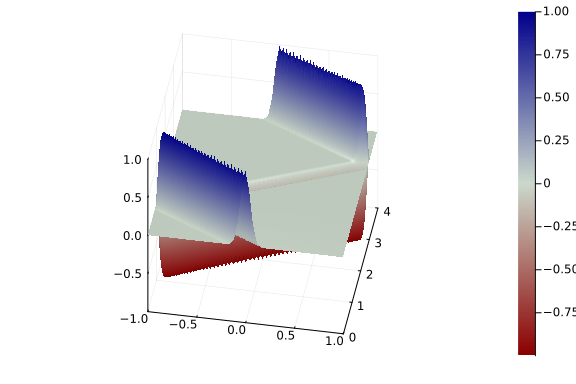
\includegraphics[width=\linewidth]{/figures/Chapter3_17_1.pdf}

\begin{lstlisting}
(*@\HLJLnf{contour}@*)(*@\HLJLp{(}@*)(*@\HLJLn{x}@*)(*@\HLJLp{[}@*)(*@\HLJLk{end}@*)(*@\HLJLoB{:-}@*)(*@\HLJLni{1}@*)(*@\HLJLoB{:}@*)(*@\HLJLni{1}@*)(*@\HLJLp{],}@*)(*@\HLJLn{tdata}@*)(*@\HLJLp{,}@*)(*@\HLJLn{plotdata}@*)(*@\HLJLp{[}@*)(*@\HLJLoB{:}@*)(*@\HLJLp{,}@*)(*@\HLJLk{end}@*)(*@\HLJLoB{:-}@*)(*@\HLJLni{1}@*)(*@\HLJLoB{:}@*)(*@\HLJLni{1}@*)(*@\HLJLp{])}@*)
\end{lstlisting}

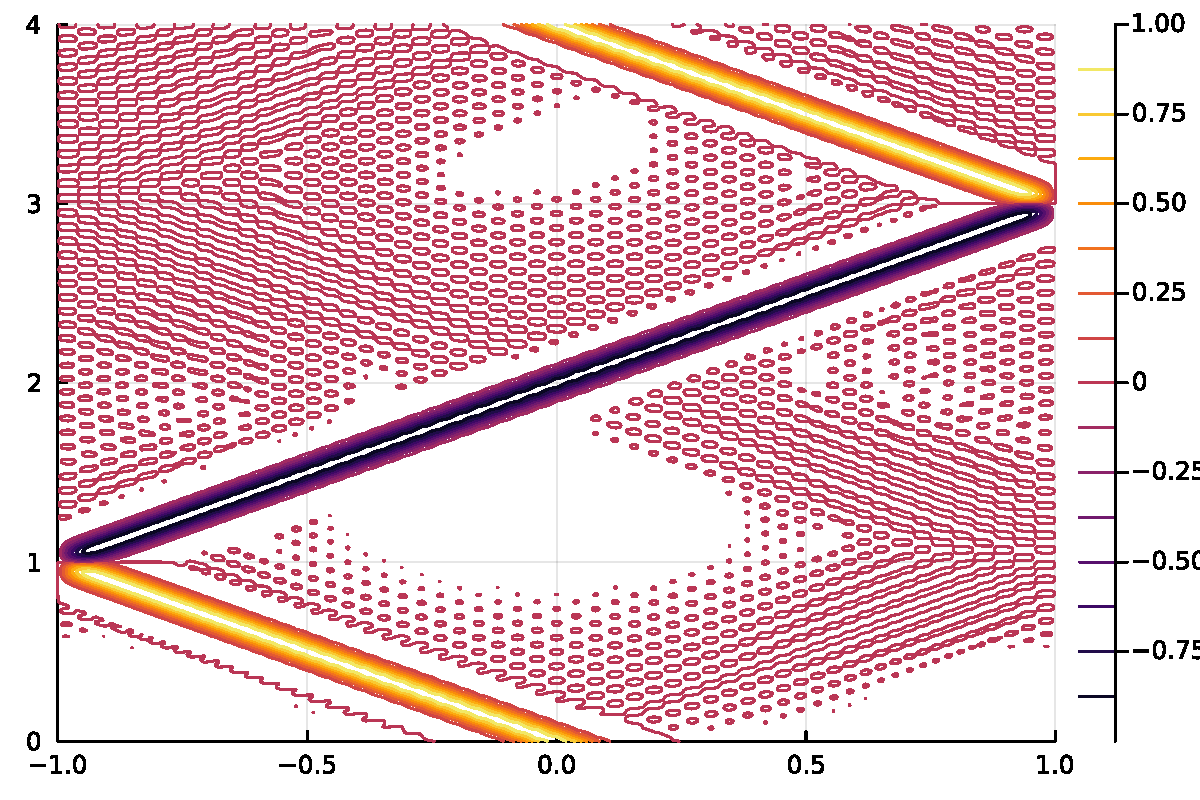
\includegraphics[width=\linewidth]{/figures/Chapter3_18_1.pdf}

\subsection{Rate of convergence of Chebyshev interpolants and their derivatives}
Since Chebyshev interpolants of a generally non-periodic function $f(x)$ on $[-1, 1]$ are trigonometric interpolants of the periodic function $g(\theta) = f(\cos\theta)$, we can deduce the rate of convergence of Chebyshev interpolating polynomials from the rate of convergence of trigonometric interpolants of $g(\theta)$.

\textbf{Examples}

\begin{itemize}
\item[1. ] For $f(x) = \vert x \vert$, $x \in [-1, 1]$, it follows that $g(\theta) = \vert \cos\theta \vert$, $\theta \in [0, \pi]$.  To apply the results we stated for periodic functions in Chapter 2, we need to consider $g$ on the interval $[0, 2\pi]$.  Since $g(\theta) \in C^{0}[0, 2\pi]$, $\| g^{(k)}\|_1 < \infty$ for $k = 0, 1, 2$ (verify) and $g^{(1)}(0), g^{(1)}(2\pi) < \infty$, it follows that

\end{itemize}
\[
\| q_{2n+1}(\theta) - g(\theta) \|_{\infty} = \| p_{n+1}(x) - f(x) \|_{\infty} = \mathcal{O}\left( n^{-1} \right), \qquad n \to \infty.
\]
where $q_{2n+1}(\theta)$ is the trigonometric interpolant of $g(\theta)$ and $p_{n+1}(x)$ is the Chebyshev interpolant of $f(x)$.

\begin{itemize}
\item[2. ] For $f(x) = \vert x \vert^3$ we want to know how fast does the derivative of the Chebyshev interpolant converge to $f'$.  Following the same reasoning as in the previous example, since $g(\theta) \in C^{2}[0, 2\pi]$, $\| g^{(k)}\|_1 < \infty$ for $k = 0, \ldots, 4$ and $g^{(3)}(0), g^{(3)}(2\pi) < \infty$, it follows that

\end{itemize}
\[
\| q_{2n+1}'(\theta) - g'(\theta) \|_{\infty} = \left\|\sqrt{1-x^2}( p_{n+1}'(x) - f'(x)) \right\|_{\infty} = \mathcal{O}\left( n^{-2} \right), \qquad n \to \infty.
\]
\begin{itemize}
\item[3. ] For $f(x) = {\rm e}^{-1/x^2}$, we have that $g(\theta) = f(\cos\theta) \in C^{\infty}[0, 2\pi]$ and thus

\end{itemize}
\[
\| q_{2n+1}(\theta) - g(\theta) \|_{\infty} = \left\| p_{n+1}(x) - f(x) \right\|_{\infty} = \mathcal{O}\left( n^{-\mu} \right), \qquad n \to \infty, 
\]
for $\mu = 1, 2, 3, \ldots$ and this rate of convergence also holds for $\| q_{2n+1}^{(\nu)}(\theta) - g^{(\nu)}(\theta) \|_{\infty}$, $\nu = 0, 1, 2, \ldots$.

\begin{itemize}
\item[4. ] For the Runge function $f(x) = 1/(1 + 25x^2)$,  $g(\theta) = f(\cos\theta)$ is analytic on $[0, 2\pi]$ and therefore $\| q_{2n+1}^{(\nu)}(\theta) - g^{(\nu)}(\theta) \|_{\infty}$ and $\| p_{n+1}^{(\nu)}(x) - f^{(\nu)}(x) \|_{\infty}$ decays exponentially fast with $n$. 


\item[5. ] For $f(x) = x^{m}$, we have that

\end{itemize}
\[
\| q_{2n+1}(\theta) - g(\theta) \|_{\infty} = \| p_{n+1}(x) - f(x) \|_{\infty} = 0
\]
for $n \geq m$ because $q_{2n+1}(\theta) = g(\theta)$ and $p_{n+1}(x) = f(x)$ for $n \geq m$.  Therefore, we also have  

\[
\| q_{2n+1}^{(\nu)}(\theta) - g^{(\nu)}(\theta) \|_{\infty} = \| p_{n+1}^{(\nu)}(x) - f^{(\nu)}(x) \|_{\infty} = 0
\]
for $\nu = 0, 1, \ldots$ if $n \geq m$.

Let's check whether the numerics agree with these predictions:


\begin{lstlisting}
(*@\HLJLn{f\ensuremath{\_1}}@*) (*@\HLJLoB{=}@*) (*@\HLJLn{x}@*) (*@\HLJLoB{->}@*) (*@\HLJLnf{abs}@*)(*@\HLJLp{(}@*)(*@\HLJLn{x}@*)(*@\HLJLp{)}@*)
(*@\HLJLn{xx}@*) (*@\HLJLoB{=}@*) (*@\HLJLnf{range}@*)(*@\HLJLp{(}@*)(*@\HLJLoB{-}@*)(*@\HLJLni{1}@*)(*@\HLJLp{,}@*)(*@\HLJLni{1}@*)(*@\HLJLp{;}@*)(*@\HLJLn{length}@*)(*@\HLJLoB{=}@*)(*@\HLJLni{1001}@*)(*@\HLJLp{)}@*) (*@\HLJLcs{{\#}}@*) (*@\HLJLcs{compute}@*) (*@\HLJLcs{the}@*) (*@\HLJLcs{error}@*) (*@\HLJLcs{on}@*) (*@\HLJLcs{this}@*) (*@\HLJLcs{grid}@*)
(*@\HLJLn{nn}@*) (*@\HLJLoB{=}@*) (*@\HLJLni{2}@*) (*@\HLJLoB{.{\textasciicircum}}@*)(*@\HLJLp{(}@*)(*@\HLJLni{4}@*)(*@\HLJLoB{:}@*)(*@\HLJLni{20}@*)(*@\HLJLp{)}@*)
(*@\HLJLn{S}@*) (*@\HLJLoB{=}@*) (*@\HLJLnf{Chebyshev}@*)(*@\HLJLp{()}@*)
(*@\HLJLcs{{\#}}@*) (*@\HLJLcs{use}@*) (*@\HLJLcs{ApproxFun}@*) (*@\HLJLcs{to}@*) (*@\HLJLcs{construct}@*) (*@\HLJLcs{and}@*) (*@\HLJLcs{evaluate}@*) (*@\HLJLcs{Chebyshev}@*) (*@\HLJLcs{interpolant}@*)
(*@\HLJLn{errs}@*) (*@\HLJLoB{=}@*) (*@\HLJLp{[(}@*) (*@\HLJLn{p\ensuremath{\_n}}@*) (*@\HLJLoB{=}@*) (*@\HLJLnf{Fun}@*)(*@\HLJLp{(}@*)(*@\HLJLn{f\ensuremath{\_1}}@*)(*@\HLJLp{,}@*)(*@\HLJLn{S}@*)(*@\HLJLp{,}@*)(*@\HLJLn{n}@*)(*@\HLJLp{);}@*)
        (*@\HLJLnf{norm}@*)(*@\HLJLp{(}@*)(*@\HLJLn{f\ensuremath{\_1}}@*)(*@\HLJLoB{.}@*)(*@\HLJLp{(}@*)(*@\HLJLn{xx}@*)(*@\HLJLp{)}@*) (*@\HLJLoB{-}@*) (*@\HLJLn{p\ensuremath{\_n}}@*)(*@\HLJLoB{.}@*)(*@\HLJLp{(}@*)(*@\HLJLn{xx}@*)(*@\HLJLp{),}@*)(*@\HLJLn{Inf}@*)(*@\HLJLp{)}@*)  (*@\HLJLp{)}@*) (*@\HLJLk{for}@*) (*@\HLJLn{n}@*) (*@\HLJLoB{=}@*) (*@\HLJLn{nn}@*) (*@\HLJLp{]}@*)
(*@\HLJLn{p}@*)(*@\HLJLoB{=}@*)(*@\HLJLnf{scatter}@*)(*@\HLJLp{(}@*)(*@\HLJLn{nn}@*)(*@\HLJLp{,}@*)(*@\HLJLn{errs}@*)(*@\HLJLp{;}@*)(*@\HLJLn{xscale}@*)(*@\HLJLoB{=:}@*)(*@\HLJLn{log10}@*)(*@\HLJLp{,}@*) (*@\HLJLn{yscale}@*)(*@\HLJLoB{=:}@*)(*@\HLJLn{log10}@*)(*@\HLJLp{,}@*)(*@\HLJLn{xlabel}@*)(*@\HLJLoB{=}@*)(*@\HLJLs{"{}n"{}}@*)(*@\HLJLp{,}@*)
(*@\HLJLn{label}@*)(*@\HLJLoB{=}@*)(*@\HLJLs{"{}Chebyshev}@*) (*@\HLJLs{interpolation}@*) (*@\HLJLs{error}@*) (*@\HLJLs{for}@*) (*@\HLJLs{f}@*) (*@\HLJLs{=}@*) (*@\HLJLs{|x|"{}}@*)(*@\HLJLp{)}@*)
(*@\HLJLnf{plot!}@*)(*@\HLJLp{(}@*)(*@\HLJLn{nn}@*)(*@\HLJLp{,}@*)(*@\HLJLni{1}@*) (*@\HLJLoB{./}@*)(*@\HLJLn{nn}@*)(*@\HLJLp{;}@*)(*@\HLJLn{label}@*)(*@\HLJLoB{=}@*)(*@\HLJLs{"{}1/n"{}}@*)(*@\HLJLp{)}@*)
\end{lstlisting}

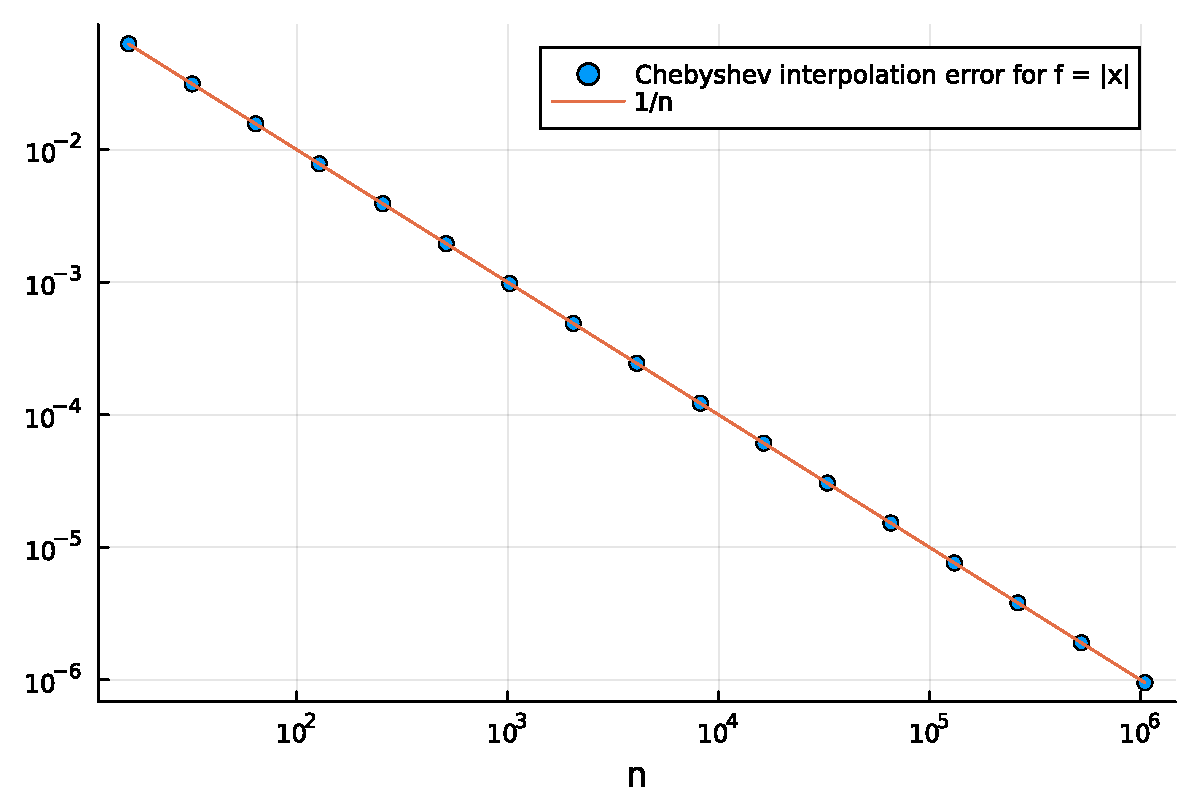
\includegraphics[width=\linewidth]{/figures/Chapter3_19_1.pdf}

\begin{lstlisting}
(*@\HLJLn{f\ensuremath{\_2}}@*) (*@\HLJLoB{=}@*) (*@\HLJLn{x}@*) (*@\HLJLoB{->}@*) (*@\HLJLnf{abs}@*)(*@\HLJLp{(}@*)(*@\HLJLn{x}@*)(*@\HLJLp{)}@*)(*@\HLJLoB{{\textasciicircum}}@*)(*@\HLJLni{3}@*)
(*@\HLJLn{df\ensuremath{\_2}}@*) (*@\HLJLoB{=}@*) (*@\HLJLn{x}@*) (*@\HLJLoB{->}@*) (*@\HLJLn{x}@*) (*@\HLJLoB{<}@*) (*@\HLJLni{0}@*) (*@\HLJLoB{?}@*) (*@\HLJLoB{-}@*)(*@\HLJLni{3}@*)(*@\HLJLn{x}@*)(*@\HLJLoB{{\textasciicircum}}@*)(*@\HLJLni{2}@*) (*@\HLJLoB{:}@*) (*@\HLJLni{3}@*)(*@\HLJLn{x}@*)(*@\HLJLoB{{\textasciicircum}}@*)(*@\HLJLni{2}@*)
(*@\HLJLn{nn}@*) (*@\HLJLoB{=}@*) (*@\HLJLni{2}@*) (*@\HLJLoB{.{\textasciicircum}}@*)(*@\HLJLp{(}@*)(*@\HLJLni{4}@*)(*@\HLJLoB{:}@*)(*@\HLJLni{18}@*)(*@\HLJLp{)}@*)
(*@\HLJLn{errs}@*) (*@\HLJLoB{=}@*) (*@\HLJLp{[(}@*) (*@\HLJLn{x}@*) (*@\HLJLoB{=}@*) (*@\HLJLn{cos}@*)(*@\HLJLoB{.}@*)(*@\HLJLp{(}@*)(*@\HLJLn{\ensuremath{\pi}}@*)(*@\HLJLoB{*}@*)(*@\HLJLp{(}@*)(*@\HLJLni{0}@*)(*@\HLJLoB{:}@*)(*@\HLJLn{n}@*)(*@\HLJLp{)}@*)(*@\HLJLoB{/}@*)(*@\HLJLn{n}@*)(*@\HLJLp{);}@*)
          (*@\HLJLnf{norm}@*)(*@\HLJLp{(}@*)(*@\HLJLn{df\ensuremath{\_2}}@*)(*@\HLJLoB{.}@*)(*@\HLJLp{(}@*)(*@\HLJLn{x}@*)(*@\HLJLp{)}@*) (*@\HLJLoB{-}@*) (*@\HLJLnf{chebfft}@*)(*@\HLJLp{(}@*)(*@\HLJLn{f\ensuremath{\_2}}@*)(*@\HLJLoB{.}@*)(*@\HLJLp{(}@*)(*@\HLJLn{x}@*)(*@\HLJLp{)),}@*)(*@\HLJLn{Inf}@*)(*@\HLJLp{))}@*) (*@\HLJLk{for}@*) (*@\HLJLn{n}@*) (*@\HLJLoB{=}@*) (*@\HLJLn{nn}@*)(*@\HLJLp{]}@*)
(*@\HLJLn{p}@*) (*@\HLJLoB{=}@*) (*@\HLJLnf{scatter!}@*)(*@\HLJLp{(}@*)(*@\HLJLn{nn}@*)(*@\HLJLp{,}@*)(*@\HLJLn{errs}@*)(*@\HLJLp{;}@*)(*@\HLJLn{xscale}@*)(*@\HLJLoB{=:}@*)(*@\HLJLn{log10}@*)(*@\HLJLp{,}@*) (*@\HLJLn{yscale}@*)(*@\HLJLoB{=:}@*)(*@\HLJLn{log10}@*)(*@\HLJLp{,}@*)(*@\HLJLn{xlabel}@*)(*@\HLJLoB{=}@*)(*@\HLJLs{"{}n"{}}@*)(*@\HLJLp{,}@*)
(*@\HLJLn{label}@*)(*@\HLJLoB{=}@*)(*@\HLJLs{"{}Chebyshev}@*) (*@\HLJLs{differentiation}@*) (*@\HLJLs{error}@*) (*@\HLJLs{for}@*) (*@\HLJLs{f}@*) (*@\HLJLs{=}@*) (*@\HLJLs{|x|{\textasciicircum}3"{}}@*)(*@\HLJLp{)}@*)
(*@\HLJLnf{plot!}@*)(*@\HLJLp{(}@*)(*@\HLJLn{nn}@*)(*@\HLJLp{,}@*)(*@\HLJLni{1}@*) (*@\HLJLoB{./}@*)(*@\HLJLn{nn}@*)(*@\HLJLoB{.{\textasciicircum}}@*)(*@\HLJLni{2}@*)(*@\HLJLp{;}@*)(*@\HLJLn{label}@*)(*@\HLJLoB{=}@*)(*@\HLJLs{"{}1/n{\textasciicircum}2"{}}@*)(*@\HLJLp{)}@*)
\end{lstlisting}

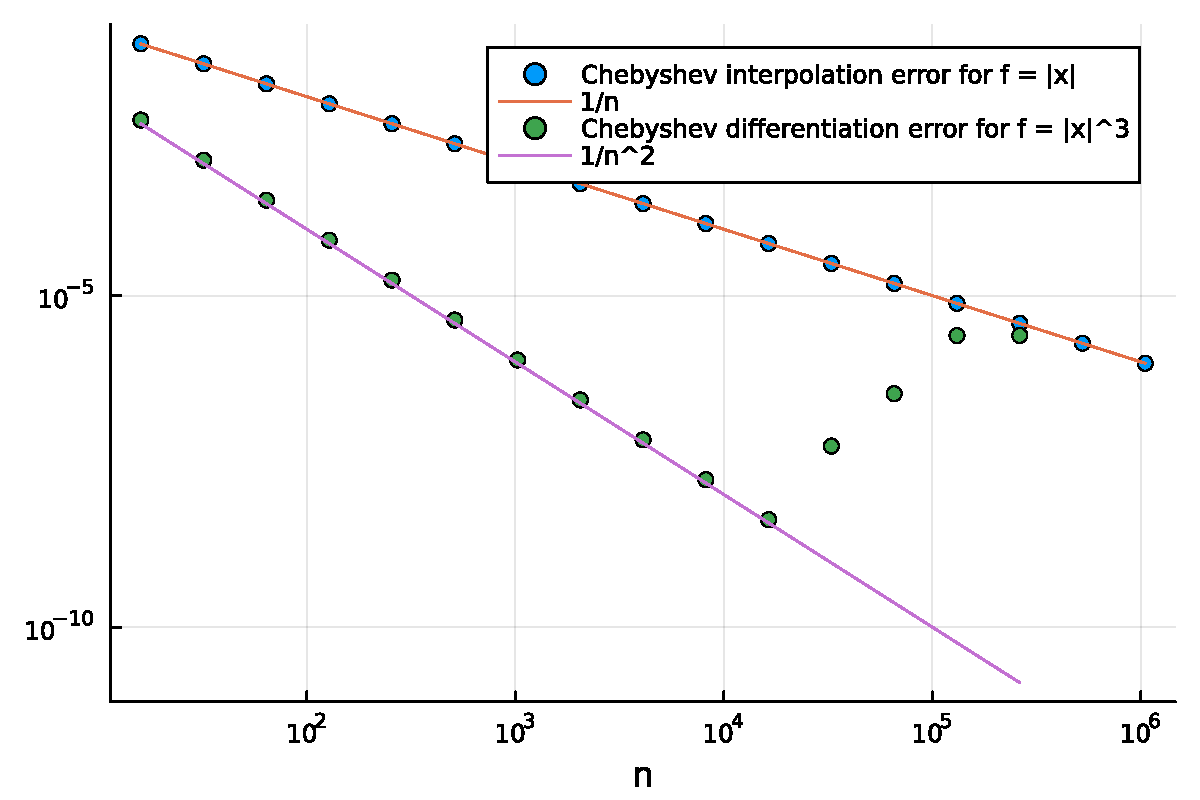
\includegraphics[width=\linewidth]{/figures/Chapter3_20_1.pdf}

The increase of the error for Chebyshev differentiation is caused by a combination of rounding errors on the order of $10^{-15}$ and the $\mathcal{O}(n^2)$ growth in the formulae for Chebyshev differentiation at $x = \pm 1$ (see the function $\texttt{chebfft}$).


\begin{lstlisting}
(*@\HLJLn{f\ensuremath{\_3}}@*) (*@\HLJLoB{=}@*) (*@\HLJLn{x}@*) (*@\HLJLoB{->}@*) (*@\HLJLnf{exp}@*)(*@\HLJLp{(}@*)(*@\HLJLoB{-}@*)(*@\HLJLni{1}@*)(*@\HLJLoB{/}@*)(*@\HLJLn{x}@*)(*@\HLJLoB{{\textasciicircum}}@*)(*@\HLJLni{2}@*)(*@\HLJLp{)}@*)
(*@\HLJLn{df\ensuremath{\_3}}@*) (*@\HLJLoB{=}@*) (*@\HLJLn{x}@*) (*@\HLJLoB{->}@*) (*@\HLJLn{x}@*) (*@\HLJLoB{==}@*) (*@\HLJLni{0}@*) (*@\HLJLoB{?}@*) (*@\HLJLni{0}@*) (*@\HLJLoB{:}@*) (*@\HLJLni{2}@*)(*@\HLJLoB{*}@*)(*@\HLJLnf{exp}@*)(*@\HLJLp{(}@*)(*@\HLJLoB{-}@*)(*@\HLJLni{1}@*)(*@\HLJLoB{/}@*)(*@\HLJLn{x}@*)(*@\HLJLoB{{\textasciicircum}}@*)(*@\HLJLni{2}@*)(*@\HLJLp{)}@*)(*@\HLJLoB{/}@*)(*@\HLJLn{x}@*)(*@\HLJLoB{{\textasciicircum}}@*)(*@\HLJLni{3}@*)
(*@\HLJLn{nn}@*) (*@\HLJLoB{=}@*) (*@\HLJLni{10}@*)(*@\HLJLoB{:}@*)(*@\HLJLni{10}@*)(*@\HLJLoB{:}@*)(*@\HLJLni{300}@*)
(*@\HLJLn{errs}@*) (*@\HLJLoB{=}@*) (*@\HLJLp{[(}@*) (*@\HLJLn{x}@*) (*@\HLJLoB{=}@*) (*@\HLJLn{cos}@*)(*@\HLJLoB{.}@*)(*@\HLJLp{(}@*)(*@\HLJLn{\ensuremath{\pi}}@*)(*@\HLJLoB{*}@*)(*@\HLJLp{(}@*)(*@\HLJLni{0}@*)(*@\HLJLoB{:}@*)(*@\HLJLn{n}@*)(*@\HLJLp{)}@*)(*@\HLJLoB{/}@*)(*@\HLJLn{n}@*)(*@\HLJLp{);}@*)
          (*@\HLJLnf{norm}@*)(*@\HLJLp{(}@*)(*@\HLJLn{df\ensuremath{\_3}}@*)(*@\HLJLoB{.}@*)(*@\HLJLp{(}@*)(*@\HLJLn{x}@*)(*@\HLJLp{)}@*) (*@\HLJLoB{-}@*) (*@\HLJLnf{chebfft}@*)(*@\HLJLp{(}@*)(*@\HLJLn{f\ensuremath{\_3}}@*)(*@\HLJLoB{.}@*)(*@\HLJLp{(}@*)(*@\HLJLn{x}@*)(*@\HLJLp{)),}@*)(*@\HLJLn{Inf}@*)(*@\HLJLp{))}@*) (*@\HLJLk{for}@*) (*@\HLJLn{n}@*) (*@\HLJLoB{=}@*) (*@\HLJLn{nn}@*)(*@\HLJLp{]}@*)
(*@\HLJLn{p}@*) (*@\HLJLoB{=}@*) (*@\HLJLnf{scatter!}@*)(*@\HLJLp{(}@*)(*@\HLJLn{nn}@*)(*@\HLJLp{,}@*)(*@\HLJLn{errs}@*)(*@\HLJLp{;}@*)(*@\HLJLn{xscale}@*)(*@\HLJLoB{=:}@*)(*@\HLJLn{log10}@*)(*@\HLJLp{,}@*) (*@\HLJLn{yscale}@*)(*@\HLJLoB{=:}@*)(*@\HLJLn{log10}@*)(*@\HLJLp{,}@*)(*@\HLJLn{xlabel}@*)(*@\HLJLoB{=}@*)(*@\HLJLs{"{}n"{}}@*)(*@\HLJLp{,}@*)
(*@\HLJLn{label}@*)(*@\HLJLoB{=}@*)(*@\HLJLs{"{}Chebyshev}@*) (*@\HLJLs{differentiation}@*) (*@\HLJLs{error}@*) (*@\HLJLs{for}@*) (*@\HLJLs{f}@*) (*@\HLJLs{=}@*) (*@\HLJLs{exp(-1/x{\textasciicircum}2)"{}}@*)(*@\HLJLp{)}@*)
\end{lstlisting}

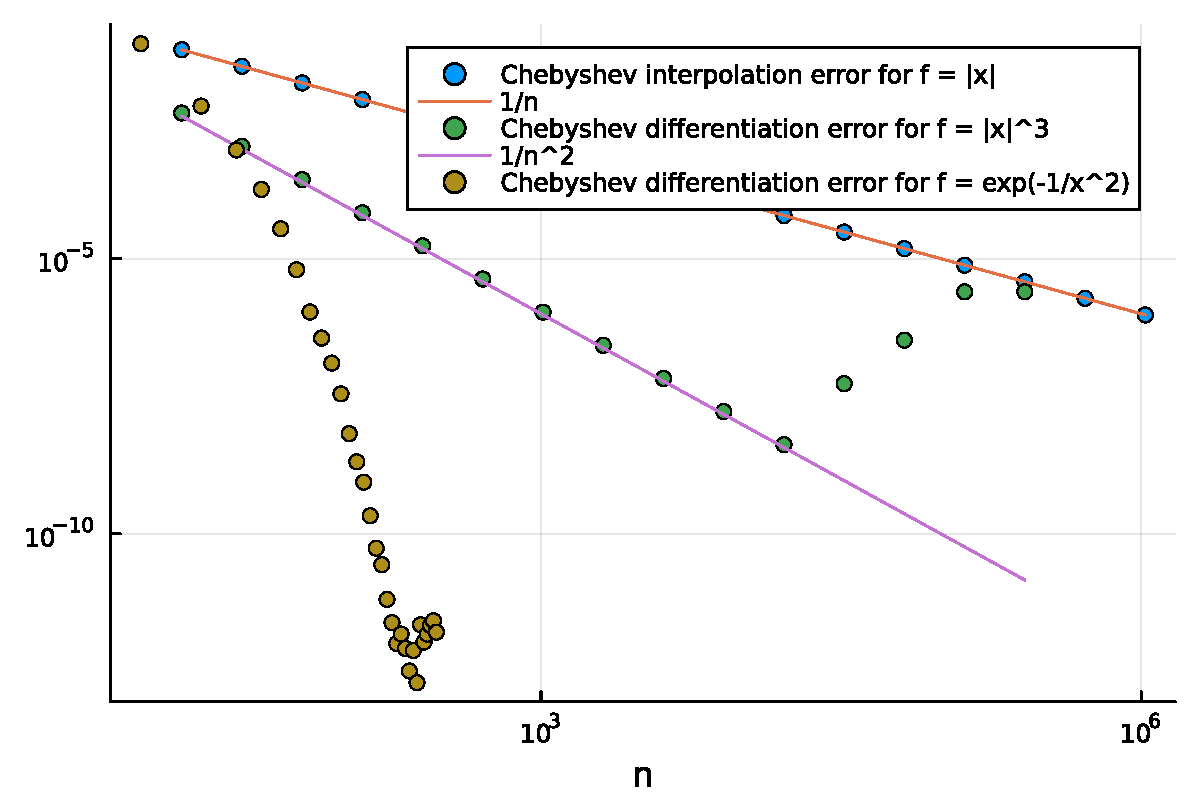
\includegraphics[width=\linewidth]{/figures/Chapter3_21_1.pdf}

\begin{lstlisting}
(*@\HLJLnf{scatter}@*)(*@\HLJLp{(}@*)(*@\HLJLn{nn}@*)(*@\HLJLp{,}@*)(*@\HLJLn{errs}@*)(*@\HLJLp{;}@*)(*@\HLJLn{yscale}@*)(*@\HLJLoB{=:}@*)(*@\HLJLn{log10}@*)(*@\HLJLp{,}@*)(*@\HLJLn{label}@*)(*@\HLJLoB{=}@*)(*@\HLJLs{"{}Chebyshev}@*) (*@\HLJLs{differentiation}@*) (*@\HLJLs{error}@*) (*@\HLJLs{for}@*) (*@\HLJLs{f}@*) (*@\HLJLs{=}@*) (*@\HLJLs{exp(-1/x\ensuremath{\^2})"{}}@*)(*@\HLJLp{)}@*)
(*@\HLJLn{f\ensuremath{\_4}}@*) (*@\HLJLoB{=}@*) (*@\HLJLn{x}@*) (*@\HLJLoB{->}@*) (*@\HLJLni{1}@*)(*@\HLJLoB{/}@*)(*@\HLJLp{(}@*)(*@\HLJLni{1}@*) (*@\HLJLoB{+}@*) (*@\HLJLni{25}@*)(*@\HLJLn{x}@*)(*@\HLJLoB{{\textasciicircum}}@*)(*@\HLJLni{2}@*)(*@\HLJLp{)}@*)
(*@\HLJLn{df\ensuremath{\_4}}@*) (*@\HLJLoB{=}@*) (*@\HLJLn{x}@*) (*@\HLJLoB{->}@*)  (*@\HLJLoB{-}@*)(*@\HLJLni{50}@*)(*@\HLJLoB{*}@*)(*@\HLJLn{x}@*)(*@\HLJLoB{/}@*)(*@\HLJLp{(}@*)(*@\HLJLni{1}@*) (*@\HLJLoB{+}@*) (*@\HLJLni{25}@*)(*@\HLJLn{x}@*)(*@\HLJLoB{{\textasciicircum}}@*)(*@\HLJLni{2}@*)(*@\HLJLp{)}@*)(*@\HLJLoB{{\textasciicircum}}@*)(*@\HLJLni{2}@*)
(*@\HLJLn{nn}@*) (*@\HLJLoB{=}@*) (*@\HLJLni{10}@*)(*@\HLJLoB{:}@*)(*@\HLJLni{10}@*)(*@\HLJLoB{:}@*)(*@\HLJLni{300}@*)
(*@\HLJLn{errs}@*) (*@\HLJLoB{=}@*) (*@\HLJLp{[(}@*) (*@\HLJLn{x}@*) (*@\HLJLoB{=}@*) (*@\HLJLn{cos}@*)(*@\HLJLoB{.}@*)(*@\HLJLp{(}@*)(*@\HLJLn{\ensuremath{\pi}}@*)(*@\HLJLoB{*}@*)(*@\HLJLp{(}@*)(*@\HLJLni{0}@*)(*@\HLJLoB{:}@*)(*@\HLJLn{n}@*)(*@\HLJLp{)}@*)(*@\HLJLoB{/}@*)(*@\HLJLn{n}@*)(*@\HLJLp{);}@*)
          (*@\HLJLnf{norm}@*)(*@\HLJLp{(}@*)(*@\HLJLn{df\ensuremath{\_4}}@*)(*@\HLJLoB{.}@*)(*@\HLJLp{(}@*)(*@\HLJLn{x}@*)(*@\HLJLp{)}@*) (*@\HLJLoB{-}@*) (*@\HLJLnf{chebfft}@*)(*@\HLJLp{(}@*)(*@\HLJLn{f\ensuremath{\_4}}@*)(*@\HLJLoB{.}@*)(*@\HLJLp{(}@*)(*@\HLJLn{x}@*)(*@\HLJLp{)),}@*)(*@\HLJLn{Inf}@*)(*@\HLJLp{))}@*) (*@\HLJLk{for}@*) (*@\HLJLn{n}@*) (*@\HLJLoB{=}@*) (*@\HLJLn{nn}@*)(*@\HLJLp{]}@*)
(*@\HLJLnf{scatter!}@*)(*@\HLJLp{(}@*)(*@\HLJLn{nn}@*)(*@\HLJLp{,}@*)(*@\HLJLn{errs}@*)(*@\HLJLp{;}@*)(*@\HLJLn{label}@*)(*@\HLJLoB{=}@*)(*@\HLJLs{"{}Chebyshev}@*) (*@\HLJLs{differentiation}@*) (*@\HLJLs{error}@*) (*@\HLJLs{for}@*) (*@\HLJLs{f}@*) (*@\HLJLs{=}@*) (*@\HLJLs{1/(1}@*) (*@\HLJLs{+}@*) (*@\HLJLs{25x\ensuremath{\^2})"{}}@*)(*@\HLJLp{)}@*)
(*@\HLJLn{f\ensuremath{\_5}}@*) (*@\HLJLoB{=}@*) (*@\HLJLn{x}@*) (*@\HLJLoB{->}@*) (*@\HLJLn{x}@*)(*@\HLJLoB{{\textasciicircum}}@*)(*@\HLJLp{(}@*)(*@\HLJLni{20}@*)(*@\HLJLp{)}@*)
(*@\HLJLn{df\ensuremath{\_5}}@*) (*@\HLJLoB{=}@*) (*@\HLJLn{x}@*) (*@\HLJLoB{->}@*)  (*@\HLJLni{20}@*)(*@\HLJLoB{*}@*)(*@\HLJLn{x}@*)(*@\HLJLoB{{\textasciicircum}}@*)(*@\HLJLni{19}@*)
(*@\HLJLn{nn}@*) (*@\HLJLoB{=}@*) (*@\HLJLni{1}@*)(*@\HLJLoB{:}@*)(*@\HLJLni{100}@*)
(*@\HLJLn{errs}@*) (*@\HLJLoB{=}@*) (*@\HLJLp{[(}@*) (*@\HLJLn{x}@*) (*@\HLJLoB{=}@*) (*@\HLJLn{cos}@*)(*@\HLJLoB{.}@*)(*@\HLJLp{(}@*)(*@\HLJLn{\ensuremath{\pi}}@*)(*@\HLJLoB{*}@*)(*@\HLJLp{(}@*)(*@\HLJLni{0}@*)(*@\HLJLoB{:}@*)(*@\HLJLn{n}@*)(*@\HLJLp{)}@*)(*@\HLJLoB{/}@*)(*@\HLJLn{n}@*)(*@\HLJLp{);}@*)
          (*@\HLJLnf{norm}@*)(*@\HLJLp{(}@*)(*@\HLJLn{df\ensuremath{\_5}}@*)(*@\HLJLoB{.}@*)(*@\HLJLp{(}@*)(*@\HLJLn{x}@*)(*@\HLJLp{)}@*) (*@\HLJLoB{-}@*) (*@\HLJLnf{chebfft}@*)(*@\HLJLp{(}@*)(*@\HLJLn{f\ensuremath{\_5}}@*)(*@\HLJLoB{.}@*)(*@\HLJLp{(}@*)(*@\HLJLn{x}@*)(*@\HLJLp{)),}@*)(*@\HLJLn{Inf}@*)(*@\HLJLp{))}@*) (*@\HLJLk{for}@*) (*@\HLJLn{n}@*) (*@\HLJLoB{=}@*) (*@\HLJLn{nn}@*)(*@\HLJLp{]}@*)
(*@\HLJLnf{scatter!}@*)(*@\HLJLp{(}@*)(*@\HLJLn{nn}@*)(*@\HLJLp{,}@*)(*@\HLJLn{errs}@*)(*@\HLJLp{;}@*)(*@\HLJLn{label}@*)(*@\HLJLoB{=}@*)(*@\HLJLs{"{}Chebyshev}@*) (*@\HLJLs{differentiation}@*) (*@\HLJLs{error}@*) (*@\HLJLs{for}@*) (*@\HLJLs{f}@*) (*@\HLJLs{=}@*) (*@\HLJLs{x\ensuremath{\^2}\ensuremath{\^0}"{}}@*)(*@\HLJLp{)}@*)
\end{lstlisting}

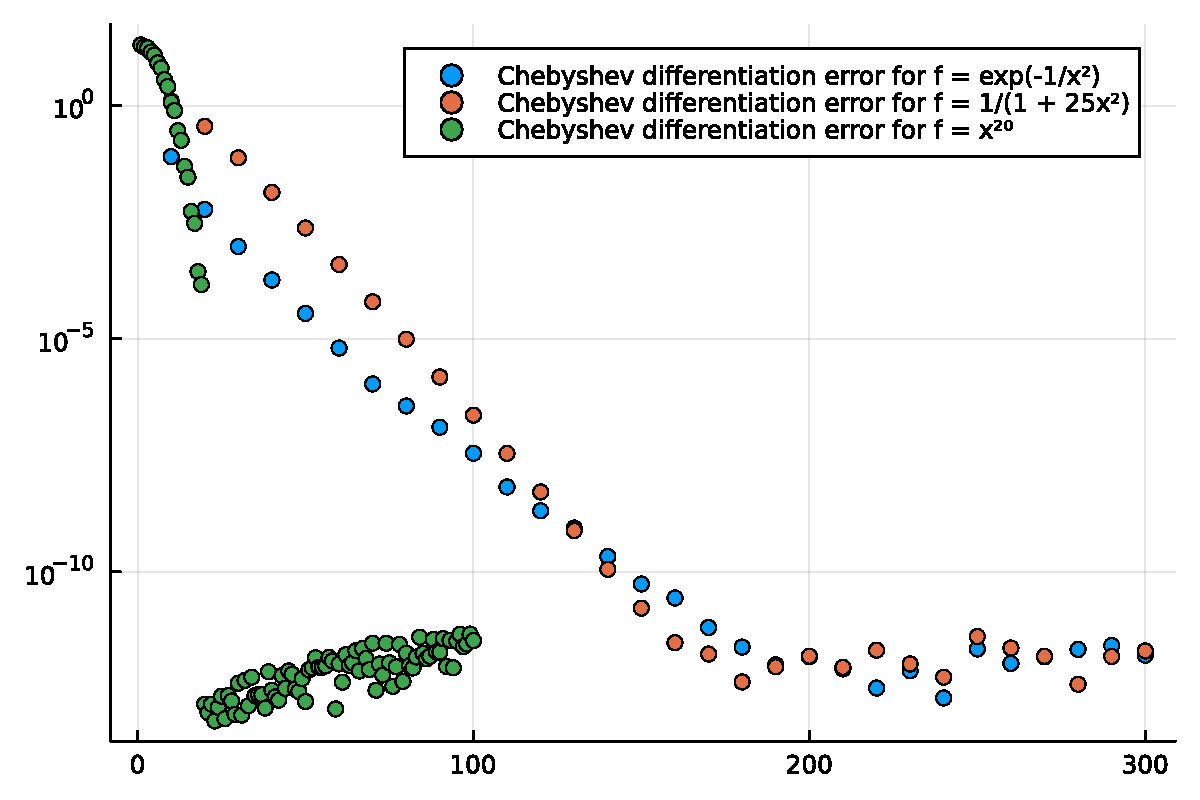
\includegraphics[width=\linewidth]{/figures/Chapter3_22_1.pdf}

Note that this a plot with semi-logarithmic axes whereas the previous plot is a log-log set of axes.



\end{document}
